% arara: pdflatex: { synctex: yes }
% arara: makeindex: { style: ctuthesis }
% arara: bibtex

% The class takes all the key=value arguments that \ctusetup does,
% and a couple more: draft and oneside
\documentclass[twoside]{casti/sablona/ctuthesis}

\ctusetup{
	preprint = \ctuverlog,
%	mainlanguage = english,
%	titlelanguage = czech,
	mainlanguage = czech,
	otherlanguages = {slovak,english},
	title-czech = {Zpracování High Density EEG signálů pro potřeby inverzní úlohy v epileptologii},
	title-english = {High Density EEG signal processing in inverse problem of epileptology},
	subtitle-czech = {},
	subtitle-english = {},
	doctype = M,
	faculty = F3,
	department-czech = {Katedra teorie obvodů},
	department-english = {Department of Circuit Theory},
	author = {Bc. Tomáš Hrstka},
	supervisor = {Ing. Radek Janča, Ph.D.},
%	supervisor-address = {Ústav X, \\ Uliční 5, \\ Praha 99},
%	supervisor-specialist = {John Doe},
%	fieldofstudy-english = {Mathematical Engineering},
%	subfieldofstudy-english = {Mathematical Modelling},
	fieldofstudy-czech = {Biomedicínské inženýrství},
	subfieldofstudy-czech = {Biomedicínské inženýrství a informatika},
	keywords-czech = {EEG, zdrojová lokalizace, inverzní úloha, zpracování signálů},
	keywords-english = {EEG, source localization, inverse problem, signal preprocessing},
	day = 27,
	month = 5,
	year = 2016,
	specification-file = {./casti/zadani/zadani.pdf},
%	front-specification = true,
%	front-list-of-figures = false,
%	front-list-of-tables = false,
%	monochrome = true,
%	layout-short = true,
}

\ctuprocess

\addto\ctucaptionsczech{%
	\def\supervisorname{Vedoucí}%
	\def\subfieldofstudyname{Studijní program}%
}

\ctutemplateset{maketitle twocolumn default}{
	\begin{twocolumnfrontmatterpage}
		\ctutemplate{twocolumn.thanks}
		\ctutemplate{twocolumn.declaration}
		\ctutemplate{twocolumn.abstract.in.titlelanguage}
		\ctutemplate{twocolumn.abstract.in.secondlanguage}
		\ctutemplate{twocolumn.tableofcontents}
		\ctutemplate{twocolumn.listoffigures}
	\end{twocolumnfrontmatterpage}
}

% Theorem declarations, this is the reasonable default, anybody can do what they wish.
% If you prefer theorems in italics rather than slanted, use \theoremstyle{plainit}
\theoremstyle{plain}
\newtheorem{theorem}{Theorem}[chapter]
\newtheorem{corollary}[theorem]{Corollary}
\newtheorem{lemma}[theorem]{Lemma}
\newtheorem{proposition}[theorem]{Proposition}

\theoremstyle{definition}
\newtheorem{definition}[theorem]{Definition}
\newtheorem{example}[theorem]{Example}
\newtheorem{conjecture}[theorem]{Conjecture}

\theoremstyle{note}
\newtheorem*{remark*}{Remark}
\newtheorem{remark}[theorem]{Remark}

% Abstract in Czech
\begin{abstract-czech}
Elektroencefalografie je důležitým nástrojem ke studiu záznamů elektrické aktivity mozku. Většina aplikací EEG však nevytěží ze záznamu všechny informace, zejména polohu zdroje aktivity v mozku. Nalezení ložisek mozkové aktivity lze dosáhnout výpočtem takzvaných inverzních úloh. Tyto metody je možné využít například k lokalizaci epileptogenní zóny, která je zodpovědná za vyvolávání spontánních záchvatů epileptických pacientů. Chirurgické odstranění epileptogenní zóny je jedním z možných způsobů léčby epilepsie. Tato léčba může pomoci pacientům s farmakorezistentní formou epilepsie, u které nezabírá léčba antiepileptiky.

Tato práce se zabývá problematikou algoritmů inverzních úloh, konkrétně podmínkami pro záznam elektroencefalogramů a měření pozic elektrod na skalpu, přímými úlohami, dostupnými modely hlavy a mozku, vybranými algoritmy inverzní úlohy a interpretací jejich výsledků. Získané znalosti jsou použity při potřebných úpravách high density EEG záznamu a při následné aplikaci algoritmů inverzních úloh SPM12 toolboxu v prostředí MATLAB. Práce porovnává správnost výsledků jednotlivých algoritmů inverzních úloh, řešených nad uměle vygenerovanými daty, u kterých je známá pozice zdroje pozorovaných EEG signálů. V poslední fázi jsou získané poznatky využity v praxi. Algoritmy jsou použity k nalezení zdrojů mozkové aktivity u reálných pacientů. Jsou vyhodnocena ložiska somatosenzorických evokovaných potenciálů (SEP), ale i ložiska zdrojů epileptické aktivity. Data byla naměřena na pacientech oddělení neurologických klinik nemocnice Motol pomocí high density systému o 256 elektrodách. 

Zvolenou problematiku řeším pomocí vhodného předzpracování, redukce a průměrování dat. S využitím SPM12 toolboxu specifikuji přímou úlohu, založenou na modelu hlavy, který je odvozen z MRI snímků pacienta. Následně využívám algoritmů inverzních úloh MN (minimal norm), LORETA, MSP (multiple sparse priors) a EBB (empirical Bayes beamformer). Výsledky lokalizace je možné zobrazit do skleněného mozku, nebo přímo do MRI snímku. Je dokonce možné využít virtuální elektrody a zobrazit elektrickou aktivitu kdekoli v mozku.

Ačkoli výsledky na testovacích subjektech potvrdily schopnosti metod nalézt konkrétní zdroje signálů, odhalily také možné limitace metod v případech přítomnosti neodstraněných artefaktů. Upozornily tak na potřebu správné interpretace výsledků u konkrétních pacientů.

Naimplementované rozšíření SPM12, pojmenované SPM Motol toolbox, bude v~budoucnu pomáhat lékařům nemocnice Motol při detekci epileptogenních zón z~EEG záznamů.
\end{abstract-czech}

% Abstract in English
\begin{abstract-english}
Electrocardiography is an important tool for studying brain electrical activity recordings, however most of the applications fail to capitalize on all of the data’s available information, particularly the location of active sources in the brain. Localizing the activity sources within the brain can be only achieved by solving the so-called inverse problem. These methods can be used to localize the epileptogenous zone, which is responsible for inducing spontaneous seizures of the epileptic patients. Surgical removal of the epileptogenous zone is a treatment that can help patients with the pharmacoresistant form of epilepsy.

This thesis deals with theory and problems of inverse task algorithms. In particular, it deals with the conditions for the electroencephalography recording and measurements of the positions of electrodes on the scalp, forward task, available forward models of the brain, selected algorithms of the inverse task and the interpretation of their results. Obtained knowledge is used during the preprocessing of high density EEG recordings, subsequently inverse task was calculated by using algorithms implemented in SPM12 toolbox. This thesis compares accuracy of the results of applied algorithms using artificially generated data, where the position of sources of EEG signals is known. In the last phase the acquired knowledge is used in practice, algorithms are used to find sources of brain activity in the real EEG recording of the epileptic patients. The activity sources are evaluated from somatosensory evoked potentials (SEPs) and epileptic EEG. Data were measured in Motol hospital using high density system with 256 electrodes.

Selected issues are solved by appropriate preprocessing, data reduction and averaging. The forward problem is specified using SPM12 toolbox and is based on the brain model, which is derived from the MRI images of the patients. Inverse problem is calculated next, via MN (minimum norm), LORETA, MSP (multiple sparse priors) and EBB (empirical Bayes beamformer) algorithms.  The results of the localization can be displayed in glass brain or directly in MRI images of the patient’s head. It is also possible to use virtual electrode to display electrical activity anywhere in the brain.

Although the results on the test subjects have confirmed the ability of methods to find the specific sources, they also revealed the limitations of these methods when artifacts are present. This indicated the need for proper interpretation of the results.

SPM12 toolbox expansion, named SPM Motol toolbox, was implemented. This software will help doctors of the Motol hospital with the detection of epileptogenic zones from EEG recordings.


\end{abstract-english}

% Acknowledgements / Podekovani
\begin{thanks}
Chtěl bych poděkovat panu Ing. Radku Jančovi, Ph.D. a panu Ing. Petru Ježdíkovi, Ph.D. za spolupráci, pravidelné konzultace a odborné vedení práce, které napomohlo vzniku této diplomové práce. 

Poděkování patří též pracovníkům nemocnice Motol za spolupráci při získávání dat. 

Děkuji i celé své rodině za podporu během studia na ČVUT.
\end{thanks}

% Declaration / Prohlaseni
\begin{declaration}
Prohlašuji, že jsem předloženou práci vypracoval samostatně a že jsem uvedl veškeré použité informační zdroje v souladu s Metodickým pokynem o dodržování etických principů při přípravě vysokoškolských závěrečných prací.

V Praze, \ctufield{day}.~\monthinlanguage{title}~\ctufield{year}

\vskip 0.4in
...............................

podpis autora práce
\end{declaration}

% Only for testing purposes
\listfiles
\usepackage[pagewise]{lineno}
\usepackage{lipsum,blindtext}
\usepackage{mathrsfs} % provides \mathscr used in the ridiculous examples

% Moje upravy
\setcounter{secnumdepth}{3}
\setcounter{tocdepth}{3}
\usepackage{amsmath}
\usepackage{forest}

\begin{document}
\maketitle



%!TEX ROOT=../../Diplomka.tex

\chapter{Úvod}
Epilepsie je neurologické onemocnění, vyskytující se přibližně u 1 \% obyvatel. Projevuje se výskytem epileptických záchvatů. V České republice je registrováno přibližně 80 000 epileptiků, z nichž cca 20~000 nedostatečně reaguje na léčbu antiepileptiky \cite{58, 57}. Záchvaty se mohou projevovat různě, např. dočasnou lehkou ztrátou kognitivních funkcí, halucinacemi, svalovými záškuby až po ztrátu vědomí s křečemi. Náhlý záchvat spojený se ztrátou vědomí je nebezpečný nejen pro jedince samotného, ale i pro jeho okolí. Proto epileptičtí pacienti nemohou např. vykonávat práce ve výškách, práce u~rotačních strojů nebo řídit. Další omezení plynou také z režimových opatření, která jsou součástí prevence epilepsie. Pacient musí dodržovat pravidelný spánkový režim a~nemůže tedy pracovat v třísměnném provozu (práce v noci), musí dlouhodobě užívat antiepileptika a nesmí požívat alkohol. Potřebná preventivní opatření tak snižují kvalitu života pacientů.

V případech těžkých farmakorezistentních epilepsií je zvažována léčba chirurgická, ta má potenciál zbavit pacienta záchvatů navždy. Operace bude úspěšná za předpokladu, že dokážeme přesně definovat zdrojovou oblast epileptiformní aktivity v pacientově mozku a tu následně odstranit bez poškození dalších funkcí mozku.
Jednou z neinvazivních možností, jak určit zdrojovou oblast epilepsie v mozku pacienta, je aplikace tzv. inverzní úlohy. Jedná se o proces, který odhaduje zdroj aktivity na základě naměřeného EEG (nebo MEG) a modelu pacientovy hlavy. 

V této diplomové práci se budu zabývat problematikou inverzních úloh a~jejich následnou aplikací. 

\section{Motivace}
Přesná lokalizace epileptogenní zóny je klíčová pro úspěšnost chirurgické léčby epilepsie. Její nedokonalé odstranění může vést k recidivě záchvatů. S~nástupem tomografických metod (MRI a CT) spolu s funkčními vyšetřeními (PET, fMRI) se zlepšuje i přesnost lokalizace epileptogenní zóny. Některé druhy epilepsie jsou však diagnostikovatelné pouze z elektrofyziologických projevů mozku měřitelných elektro- nebo magneto-encefalografií. Pro velmi přesné prostorové i časové rozlišení se využívá invazivního EEG, které s~sebou však nese všechna rizika spojená s operací mozku (infekce, nitrolební krvácení, otoky). Standardní EEG je, oproti invazivnímu, nerizikové a aplikací inverzních úloh jsme schopni lokalizovat epileptogenní zónu i z něho. Teorie inverzních úloh je v klinické praxi málo rozšířená, a to i přes svůj nesporný potenciál. Z tohoto důvodu se zabývám teorií a aplikací inverzních úloh ve své diplomové práci. Snažím se vytvořit jednoduchý nástroj pro výpočet inverzního problému, který by umožnil rozšíření této nerizikové metody do klinické praxe. Z rozšíření inverzních úloh mohou profitovat nejen doktoři, ale především pacienti.


\section{Cíle a požadavky práce}
V teoretické části se budu zabývat epilepsií samotnou, problematikou pořízení EEG signálů, možnostmi definování přímé úlohy a modelu pacientovy hlavy, existujícími algoritmy inverzních úloh a správností jejich výsledků. Porovnám také správnost výsledků různých algoritmů inverzních úloh, dostupných v~SPM12 toolboxu.

Ve spolupráci s Neurologickou klinikou a Klinikou dětské neurologie v~nemocnici Motol, s Ing. Petrem Ježdíkem, Ph.D. a s Ing. Radkem Jančou, Ph.D. se snažím navrhnout metody pro jednoduchou aplikaci inverzní úlohy na naměřená EEG data. Metody umožňují aplikovat potřebné procedury předzpracování signálů. Převádějí data do souborů, které jsou kompatibilní s~SPM12 toolboxem, instruují SPM12 toolbox při definici přímé úlohy a~aplikaci inverzní úlohy a následně umožňují vizualizaci výsledků buď v modelu pacientova mozku, nebo přímo v MRI snímcích.

Vytvořené nástroje použiji v poslední části ke zpracování případů vybraných pacientů, výsledky porovnám s klinickým hodnocením.


%!TEX ROOT=../../Diplomka.tex

\chapter{Teoretická část}

\section{Epilepsie}
Epilepsie je název pro soubor mozkových onemocnění charakterizovaných převážně recidivujícími a nepředvídatelnými výpadky normální mozkové aktivity, takzvanými epileptickými záchvaty. Epilepsie souhrnně označuje celou řadu mozkových dysfunkcí, které mohou mít různé příčiny na základě vrozených nebo získaných poruch.
\cite{1}

Podle definice zavedené International League Against Epilepsy (ILAE) a~International Bureau for Epilepsy (IBE) je epilepsie onemocněním mozku, které je charakteristické trvalou náchylností vytvářet epileptické záchvaty. Ty mají neurobiologické, kognitivní, psychologické a sociální důsledky. Epileptický záchvat je přechodný výskyt příznaků a/nebo symptomů, způsobených abnormálně vysokou nebo synchronní aktivitou neuronů v mozku, nebo nekontrolovanými elektrickými výboji v šedé kůře mozkové. Záchvaty přetrvávají několik sekund, minut, výjimečně hodin. Po odeznění záchvatu, v mezizáchvatovém období, může být nemocný zcela bez obtíží. \cite{2,1}

Epileptický záchvat je přechodný, s jasně viditelným nástupem a někdy méně zjevným koncem, což je způsobeno postiktálním stavem. Začátek a~konec epileptického záchvatu lze určit z chování jedince nebo EEG průběhů, nicméně tato dvě kritéria se nemusí vždy přesně shodovat. \cite{1}

Kognitivní dysfunkce se během záchvatu může projevovat jako problém s~vnímáním, pozorností, emocemi, pamětí, řečí nebo apraxií.

Abychom mohli diagnostikovat epilepsii u pacienta, je nutné, aby prožil alespoň jeden epileptický záchvat. Nestačí pouze rodová náchylnost k epilepsii nebo výskyt epileptiformních abnormalit v EEG. \cite{1}

Obecně se onemocnění objevuje ze dvou příčin. Může se jednat o již vrozenou vadu (primární epilepsie, způsobená nepříznivými vlivy během vývoje embrya), nebo o epilepsii získanou (sekundární, způsobenou pozdějším poškozením mozku úrazem, nádory apod.). Příčinou epileptických záchvatů může být jakákoliv léze mozku, která neurony částečně poškodí, ale úplně nezničí. Může se jednat i o dysfunkce v důsledku systémové poruchy, jako například hypoglykémie a hypoxie, nebo o důsledek úrazu mozku. \cite{2}

Základním patogenetickým mechanismem je epileptické ložisko (fokus, ohnisko). Jde o různě rozsáhlou populaci neuronů s patologickou elektrickou aktivitou. Patologie spočívá v porušení stavu klidové polarizace a v akční depolarizaci povrchové membrány neuronu, což způsobuje jeho hyperexcitabilitu. V ložisku dochází k abnormálním neuronálním výbojům s opakovanými salvami relativně vysokých a za sebou jdoucích potenciálů. Záchvaty mohou být ohraničené, nešíří se do okolí a klinická symptomatika je dána jejich lokalizací. V jiných případech se mohou šířit do celého mozku. \cite{2}

Přibližně 60 \% pacientů s epilepsií (0,4 \% populace) trpí nemocí kvůli epileptickému ložisku a 4,5 \% farmakorezistivních epileptiků by mohlo profitovat z operativního odstranění tohoto ložiska. Jak reportují různá epileptologická centra, za předpokladu, že dokáží přesně definovat a provést resekci epileptického ohniska, 30 – 85 \% (průměrně 60 \%) pacientů zůstává po zákroku bez záchvatů. \cite{6,4}

Důležitou roli v diagnostice epilepsie hraje EEG, v mezizáchvatovém období má význam především nález specifických grafoelementů, mezi které počítáme hroty, ostré vlny a komplexy hrot-vlna. Negativní nález v EEG však epilepsii nevylučuje. Moderní metodou je dlouhodobé video-EEG monitorování, kde současně zaznamenáváme EEG a klinické projevy. Pro zjištění strukturální léze a příčiny epilepsie jsou nejdůležitější CT a MRI, při podezření na arteriovenózní malformaci i angiografie. \cite{2}

V současnosti se typy záchvatů dělí dle oblasti mozku, která je abnormní aktivitou postižena. Toto dělení však není konečné \cite{71}:

\begin{itemize}
\item \textbf{Jednoduché parciální záchvaty } – postihují malé ložisko mozku, mohou se projevovat například poruchami smyslů, záleží na postižené oblasti mozku. Pacient zůstává při vědomí.
\item \textbf{Komplexní parciální záchvaty } – postihují rozsáhlou oblast mozku, způsobují automatický pohyb, narušují vědomí.
\item \textbf{Generalizované záchvaty bez křečí} – postihují celý mozek, jsou spojeny s krátkými výpadky vědomí, zahleděním se.
\item \textbf{Generalizované záchvaty s křečemi} – několikaminutové výpadky vědomí spojené typicky s pádem pacienta a tonickou křečí.
\end{itemize}

\subsection{Terapie}
Léčba epilepsie spojuje pravidelné dlouhodobé podávání antiepileptik s dodržování příslušné životosprávy (je třeba dodržovat pravidelný rytmus spánku a~bdění, nespat během dne, nepřijímat jednorázově velké množství tekutin, nepít alkohol a držet katogenní dietu). Podávání antiepileptik musí být pravidelné, lék nesmí být náhle vysazen a jeho dávkování je vždy řízeno odborníkem. \cite{2}

Pro těžké refrakterní epilepsie jsou dnes k dispozici antiepileptika tzv. III. generace. Některé dobře definované ložiskové epilepsie lze léčit i chirurgicky \cite{3}. Prognóza správně léčené epilepsie je celkem příznivá, záchvaty se většinou daří kompenzovat a zejména u dětí lze docílit i úplného vyléčení. \cite{2}

\subsection{Epileptologické zóny}
V současné době se již na epilepsii nahlíží jako na onemocnění zasahující spíše komplexní neurální sítě, nežli na jednotlivé ohraničené oblasti, tzv. zóny. Diagnostické metody definují zóny a léze na kortexu. Úspěšnost chirurgické léčby závisí na odstranění kritických částí epileptické sítě, zejména pak epileptogenní zóny, ve které dochází primárně k rozvoji záchvatů. Jednotlivé zóny jsou dnes dobře popsány a budu se jim věnovat v dalších podkapitolách. \cite{4}

\begin{figure}[!h]
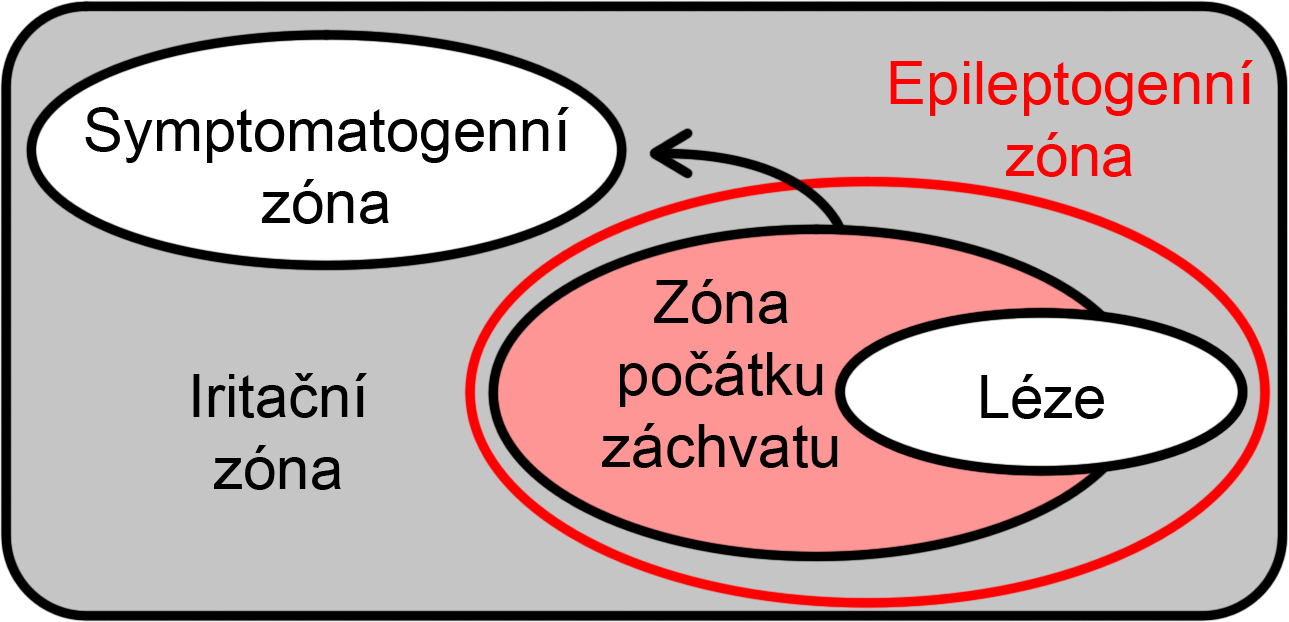
\includegraphics[scale = 0.2]{casti/teorie/zony.png}
\caption{Epileptologické zóny}
\end{figure}

\subsubsection{Symptomatogenní zóna}
Symptomatogenní zóna je část kortexu, která po aktivaci epileptoforním výbojem produkuje iktální symptomy. Tuto zónu je možné lokalizovat na základě iktální symptomatologie nebo pomocí analýzy video-EEG záznamu. Tato zóna se ve většině případů nepřekrývá s epileptogenní zónou, často však bývá s epileptogenní zónou propojena nebo se nachází v její těsné blízkosti. Nejpřesnější metodou určování pozice této zóny je přímá elektrická stimulace kortexu během invazivní explorace elektrodami. Tato procedura simuluje podobné podmínky jako při aktivaci epileptoformními výboji. \cite{4}

\subsubsection{Iritační zóna}
Tato zóna je definována jako část tkáně kortexu, generující typické mezizáchvatové výboje. Lokalizace této zóny se provádí pomocí EEG (skalpového nebo intrakraniálního), magnetoencefalografií nebo pomocí funkční magnetické rezonance (fMRI) spojené s EEG. Iritační zóna je často velmi rozsáhlá, může postihovat celou hemisféru. Její odstranění proto není nezbytně nutné, i když její zahrnutí do resekce zvyšuje šanci na dobrý pooperační výsledek. \cite{4}

\subsubsection{Zóna počátku záchvatu}
Zóna počátku záchvatu je klíčová část kortexu, ze které jsou spouštěny záchvaty a tvoří klíčovou část tzv. epileptogenní zóny. Nejčastěji lze určit její pozici z intrakraniálního EEG (vyjímečně ze skalpového EEG, lépe z~high density EEG), nebo pomocí SPECT (single photon emission computed tomografy). Skalpové EEG nám dokáže odhalit pouze přibližnou lokaci této zóny kvůli velkým plochám elektrod, jejich relativně malé citlivosti a kvůli relativně velké vzdálenosti od kortexu. Invazivní EEG je naopak velmi citlivé a zónu přesně určí pouze za předpokladu, že se elektroda nachází přímo uvnitř nebo nad touto oblastí. \cite{4}

\subsubsection{Epileptogenní strukturální léze}
Jde o abnormální mozkovou strukturu, která přímo způsobuje epilepsii. Nejčastěji je odhalena pomocí magnetické rezonance s vysokým rozlišením. Ne všechny léze na pacientově mozku jsou ovšem epileptogenní a nemusí s~epilepsií souviset. U nalezených lézí je nutné pomocí EEG ověřit, zda se jedná o~lézi zodpovědnou za pacientovy záchvaty. Dříve se mělo za to, že pouze úplná resekce takové léze vede k uzdravení pacienta. Objevily se však nové případy, ve kterých pomohla i pouze částečná resekce léze, čímž došlo k porušení klíčové struktury epileptické sítě. Na druhou stranu existují i případy, kdy ani celková resekce léze nepomohla. \cite{4}

\subsubsection{Zóna funkčního deficitu}
Zóna funkčního deficitu je část kortexu s abnormální funkčností v mezizáchvatovém období. Existuje více metod, jak určit funkčnost mozkové tkáně, a~to například pomocí psychologických a neurologických vyšetření, EEG, fMRI nebo SPECT. \cite{4}

\subsubsection{Epileptogenní zóna}
Epileptogenní zóna je pouze teoretickým konceptem, protože nelze určit její přesnou hranici. Je však zodpovědná za generování epileptických záchvatů. Pokud je pacient po operaci bez záchvatů, říkáme, že resekovaná oblast obsahovala epileptogenní zónu. \cite{4}

\subsubsection{Elokventní zóna}
Elokventní zóna je část kortexu, která brání úplné resekci epileptogenní zóny, protože plní nějakou významnou funkci jako je zrak nebo řeč. Poškození této zóny by vedlo k výraznému snížení kvality života pacienta. Zóna je lokalizována pomocí evokovaných potenciálů, MEG, fMRI nebo PET. \cite{4}




\section{Elektrofyziologická aktivita mozku}
Lidský mozek je nejkomplexnější organizovaná struktura, skládající se z cca 10\textsuperscript{10} neuronů v nejsvrchnější části v cerebrálním kortexu. Tyto buňky jsou aktivní jednotky obrovské signálové sítě, která zahrnuje 10\textsuperscript{14} propojení neboli synapsí. Během zpracovávání informací, tečou mozkem malé proudy, které můžeme měřit, tak je tomu v případě elektroencefalogramu (EEG). Můžeme také využít magnetické pole, které proudy vyvolávají (řádově fT), měřitelného pomocí magnetoencefalogramu (MEG). \cite{5}

\subsection{Magnetoencefalografie}
Počátky magnetoencefalografie se datují do šedesátých let dvacátého století, kdy se Cohen pokoušel měřit magnetické pole srdce a mozku pomocí měděných folií navinutých na feromagnetické jádro \cite{7}. Průlom přišel s vynálezem magnetometrů SQUID (superconducting quantum interference device), využívajících kvantový fenomén, nastávající při velmi nízkých teplotách, takzvaný Josephsonův jev. \cite{8}

Magnetoencefalograf je schopen zaznamenávat velmi slabá magnetická pole v řádech 10\textsuperscript{-15} Tesla (o několik řádů slabší než magnetický šum prostředí), která korelují s aktivitou neuronů v mozku. Jelikož je magnetické pole mozku tak slabé, jeho záznam je možný pouze v magneticky odstíněných místnostech \cite{6}. Fyzikální principy, na kterých MEG staví, jsou popsány v knize \cite{9}. 

Moderní MEG skenery s několika stovkami senzorů poskytují jemné prostorové rozlišení neuromagnetické aktivity mozku, díky čemuž je možné tvořit hypotézy o místech vzniku této aktivity \cite{6}. Na magnetoencefalografická data je také možné aplikovat algoritmy inverzních úloh. Proces je vcelku stejný, liší se pouze model přímé úlohy. 

MEG není předmětem této práce, nicméně jej uvádím pro úplnost.

\subsection{Elektroencefalografie}
EEG signál je záznamem potenciálů, vyvolaných proudy, které protékají během synaptické excitace dendrity neuronů cerebrálního kortexu a je následně promítán skrze pacientovu lebku až k elektrodám zaznamenávacího zařízení. EEG je typicky měřeno v řádech 10\textsuperscript{-6} voltů. Proudy v mozku jsou generovány převážně přechodem pozitivně nabitých iontů sodíku, draslíku a~vápníku a~negativně nabitých iontů chloru membránami neuronů \cite{10}. Elektrická aktivita mozku se dělí do dvou tříd: akční potenciály (AP) a postsynaptické potenciály (PSP). PSP se objeví při vyplavení neurotransmiteru presynaptickým neuronem. Dojde ke změně koncentračního gradientu, a tím ke změně membránového potenciálu. Velikost potenciálu jednoho izolovaného PSP je přímo úměrná počtu receptorů, které navázaly mediátor. Amplituda měřeného PSP klesá se vzdáleností od elektrod zaznamenávajícího přístroje. AP vzniká, jestliže membránový potenciál neuronu přesáhne jeho vnitřní prahovou hodnotu. AP se rychle šíří membránou neuronu, jeho amplituda neklesá díky napěťově citlivým sodíkovým a draslíkovým kanálkům. \cite{12}

Lidská lebka je tvořena mnoha různými vrstvami, jako jsou například skalp nebo lebka. Lebka signály generované mozkem tlumí asi stokrát víc, než ostatní měkké tkáně, proto jsme schopni zaznamenávat pouze signály větší populace aktivních neuronů. \cite{10}

Mozek také generuje signály o různých frekvencích. Jednotlivá pásma jsou označena jako delta (frekvence nižší než 4 Hz), théta (4-8 Hz), alfa (8-13 Hz), beta (13-30 Hz) a gama (30-45 Hz). \cite{10,11} Jednotlivá označení pásem jsou historická, dělená dle dominantní frekvence viditelné v EEG záznamu a~nereprezentují skutečné frekvenční spektrum EEG záznamů.  

Během epileptického záchvatu se v EEG signálu objeví výrazné změny, způsobené synchronní aktivitou neuronů. Jednou z charakteristik iktálního EEG je přítomnost hrotů a ostrých vln. Detekování záchvatů v EEG je potřebné nejen pro diagnózu, ale i pro terapii. \cite{14}

MEG a EEG je měření stejné mozkové aktivity, rozdílná je pouze pozorovaná veličina, kterou vyvolávají mozkem tekoucí proudy. Některé metody zpracování je tedy možné využít pro MEG i EEG, datový soubor je poté označován jako M/EEG nebo jen MEEG.

\subsubsection{Zpracování EEG signálu}
Časové a prostorové rozlišení (vysoká vzorkovací frekvence, velké množství elektrod) se obecně považuje za dobrou vlastnost, přináší to s sebou ovšem komplikaci v podobě množství dat, která jsou během měření signálu nasbírána. Nutností jsou tedy metody, umožňující detekovat události relevantní pro zpracování inverzní úlohy. Snažíme se z dat vyextrahovat takzvané ERP (event related potencials), EEG signál v časovém okně okolo nastalé události, na kterou chceme aplikovat inverzní úlohu. Události se mohou v datech objevovat náhodně (jako komplexy hrot-vlna u epileptiků), nebo periodicky (typicky u evokovaných potenciálů). Získané ERP jsou následně průměrovány, čímž je odstraněna náhodná aktivita, vyskytující se v jednotlivých ERP. Inverzní úloha je poté aplikována na zprůměrovaný signál.

\subsubsection{Artefakty}
EEG záznam je typicky zatížen šumy různých původů, takzvanými artefakty. Artefakty jsou nechtěné části signálu, které jsou způsobeny jinými zdroji, ne mozkem, a proto je nutné je v každém signálu identifikovat. Artefakty jsou nejčastěji způsobeny těmito zdroji:

\begin{itemize}
\item \textbf{Oční artefakty} – jsou způsobeny okohybnými svaly při pohybu očí nebo mrkání.
\item \textbf{Svalové artefakty} – interference s EMG, tyto signály zabírají širokou část frekvenčního pásma, může se jednat o rychlé hroty nebo delší oscilace.
\item \textbf{Artefakty srdeční aktivity} – interference s EKG, artefakty způsobené depolarizací srdce.
\item \textbf{Interference s rozvodnou sítí} – jedná se o naindukovaný signál rozvodné sítě o frekvenci 50 Hz nebo 60 Hz (a jejich vyšší harmonické) podle místního standardu.
\item \textbf{Pohyb elektrod} – pacientovým pohybem může dojít ke změně polohy elektrod a tím ke změně půlčlánkového potenciálu mezi skalpem a~elektrodou.
\item \textbf{Ostatní artefakty} – mohou se objevovat artefakty spojené se změnou půlčlánkového potenciálu, způsobené pocením pacienta nebo vysycháním vodivého gelu. Existují také elektrostatické artefakty, artefakty způsobené pohybem jazyka a mnoho dalších.
\end{itemize}

Jakmile identifikujeme části dat, obsahujících artefakty, můžeme buď taková data z dalšího zkoumání vyřadit, nebo některé typy artefaktů lze potlačit pomocí odpovídajících metod. \cite{13}

Nejčastější metody pro detekci artefaktů jsou založeny na lineární regresi a~snaží se eliminovat nejčastější artefakty, způsobené očními pohyby a mrkáním pomocí měření elektrookulogramu (EOG). \cite{15}

Komplexnější metody mohou být založeny na lineární dekompozici vícekanálového EEG. Takové metody předpokládají, že zdroj artefaktů a zdroj EEG jsou nezávislé a snaží se získat původní průběhy, pouze z EEG záznamu. \cite{15}

Artefakty je také možné klasifikovat pomocí klasifikátorů, tedy na základě příznaků, kterými je možné signál popsat. Příznaky je možné rozdělit do těchto kategorií:

\begin{itemize}
\item Statistické charakteristiky jako „špičatost“ (šikmost), entropie, trend a~extrémy. Špičatost lze použít pro detekci hrotů, charakteristických pro některé typy artefaktů (EOG, EKG), artefakt je indikován i vysokou hodnotou entropie během krátkého časového intervalu. \cite{16}
\item Pomocné měřené signály, pokud jsou k dispozici. Artefakt může být indikován pomocí vysoké hodnoty korelace EEG s EOG nebo EKG. \cite{17}
\item Frekvenční charakteristiky – zdroje signálu jsou často charakteristické svou energií v různých frekvenčních pásmech. \cite{17}
\item Amplituda signálu, promítnutého na skalpu, může indikovat jeho původ. \cite{18}
\end{itemize}

\subsubsection{Volba umístění a počtu elektrod}
Jednou ze zásadních otázek je, kolik elektrod je potřeba pro přesné určení zdroje aktivity. Teoreticky, čím víc elektrod, tím lepší prostorové rozlišení a~tedy přesnější výsledek. Některé články však ukázaly, že optimální rozdělení elektrod je s dvou- až třícentimetrovými rozestupy tak, aby rovnoměrně pokrývaly povrch hlavy. \cite{29,32,31}

Výsledky simulací ukazují, že vliv počtu elektrod na přesnost lokalizace zdroje signálu není lineární, přesnost roste od 25 do cca 100 elektrod (to závisí na zvolené metodě inverzní úlohy), poté přechází v plateau fázi. Simulace byla provedena naměřením EEG na 14 epileptických pacientech, EEG záznamy byly následně redukovány na nižší počty elektrod, tak aby rozestupy zůstaly uniformní.\cite{33}

\begin{figure}[!h]
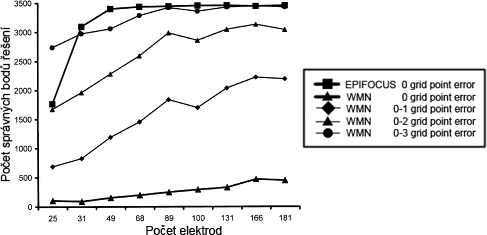
\includegraphics[scale=0.6]{casti/teorie/chybyInverze.png}
\caption{Přesnost výsledku inverzní úlohy v závislosti na počtu kanálů EEG záznamu \cite{72}}
\end{figure}

Pro algoritmus EPIFOCUS bylo dosaženo maximální přesnosti už při 68 elektrodách. Algoritmus WMN (weighted minimum norm) dosahoval nižší přesnosti lokalizace, proto byly zahrnuty i počty správných řešení pro různé rozsahy tolerancí, maximální přesnosti bylo však vždy dosaženo pro 166 elektrod. \cite{33}

Některé články navrhovaly, že pro zlepšení prostorového rozlišení v místě, kde se předpokládá přítomnost zdroje signálů, by se měla zvýšit koncentrace elektrod \cite{34}. To mělo hlavně vyřešit problém s nízkým počtem elektrod systémů 10-20. Novější články argumentují tím, že dnes již jsou systémy s dostatečně velkým počtem elektrod levné a dostupné a některé dokonce vyvracejí navržený nápad vlastními výzkumy.

\begin{figure}[!h]
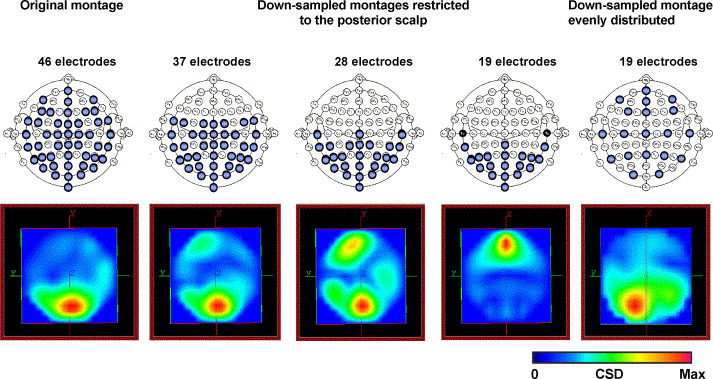
\includegraphics[width=1.0\textwidth]{casti/teorie/rozlozeniElektrod.jpg}
\caption{Vliv nerovnoměrného rozmístění elektrod na pacientově skalpu \cite{73}}
\end{figure}

Při zkoumání efektu rozdělení elektrod na lokalizaci zdroje bylo využito algoritmu Loreta v 3-shell sphere modelu hlavy (viz \ref{3-shell-sphere}). Inverzní úloha byla aplikována na vizuální evokované potenciály, aktivita je tedy očekávána v~okcipitální oblasti mozku. Lokalizace byla nejprve provedena na systému se 46 rovnoměrně rozmístěnými elektrodami (vlevo). V dalších pokusech byly vyřazovány elektrody z frontální oblasti. V posledním případě (vpravo) je zobrazen set s 19 rovnoměrně rozmístěnými elektrodami a aktivita se opět objevuje v předpokládané oblasti. Pro aplikaci inverzních úloh je tedy nutné zachovat rovnoměrné rozmístění elektrod. 


\subsubsection{Volba reference}
Nutnost volby reference je brána jako jedna z nevýhod EEG oproti MEG, aktivní reference může vést k problémům při interpretaci dat. \cite{36,37}

Pro výpočty inverzní úlohy pomocí SPM12 je nutné zaznamenat EEG signál pomocí referenčního zapojení. Jako reference může být použita některá z~elektrod (umístěná například na ušní boltec nebo kořen nosu), nebo je možné využít průměrné reference (referenční hodnota je vypočtena jako průměr hodnot všech elektrod). Dokumentace SPM12 dokonce doporučuje, aby byla data vždy pro jistotu přereferencována na průměrnou referenci, aby byly splněny předpoklady, ze kterých vychází výpočet inverzního problému. \cite{35} 

Podle \cite{38} je však volba reference u unipolárního zapojení irelevantní, protože různé reference nemění vztah mezi jednotlivými elektrodami. Mění pouze aditivní konstantu, která však nemá žádný fyzikální význam. Ekvipotenciální mapy se nijak nemění.

Bipolární záznam poskytuje měření lokálního zdroje, které je nevhodné pro účely inverzní úlohy, protože reprezentují měření skalpového proudu pouze ve směru bipolárního páru. \cite{31}


\subsubsection{Možné chyby měření}
Jednou z chyb, se kterou se můžeme setkat, je nepřesnost při snímání pozic elektrod digitizérem. Vliv nepřesné lokalizace elektrod byl testován v \cite{39}, kde byla simulována nepřesnost snímání elektrod náhodnými posuny v okruhu do 1 centimetru. Studie ukázala, že vliv této nepřesnosti na správnost výsledku inverzní úlohy je malý a oproti chybě, způsobené šumem v datech, zanedbatelný.

Další chybou, se kterou se můžeme v praxi setkat, je kanál kontaminovaný artefakty kvůli špatnému kontaktu se skalpem pacienta nebo kvůli chybě zesilovače. Takové elektrody je možné z inverzní úlohy jednoduše vyřadit, aniž by byla ovlivněna přesnost lokalizace aktivní oblasti mozku. \cite{29}





\section{Zdrojová analýza}
Během posledních několika dekád bylo vyvinuto velké množství technik vyhodnocování neinvazivního měření mozkové aktivity. Jednou z nich je zdrojová analýza, jejíž snahou je z elektroencefalografických (EEG) nebo magnetoencefalografických (MEG) dat (souhrnně označovaná jako M/EEG) lokalizovat zdroj pozorované aktivity. Na naměřená data jsou aplikovány techniky zpracování signálu s~cílem odhadnout proudové zdroje v mozku tak, aby bylo dosaženo nejlepší shody s naměřenými daty. Tento proces se nazývá inverzní úloha. \cite{20}

Metody zdrojové analýzy mohou být využity v epileptologii. Výsledky algoritmů jsou schopny správně lokalizovat epileptogenní zónu. Tato problematika je předmětem zkoumání mnoha článků, příkladem jsou \cite{59}, \cite{60}, \cite{62} nebo \cite{33}.

Prvním krokem zdrojové lokalizace je snaha nalézt skalpové potenciály, vyvolané hypotetickými proudovými dipóly, nebo obecněji distribucí proudů. Jinými slovy, definujeme, jaké EEG signály vyvolá aktivace daného místa v~mozku. Tento krok se nazývá přímá úloha (forward problem) a je nedílnou součástí výpočtu inverzní úlohy \cite{19}. Pomocí modelu, vzniklého při vypočtu přímé úlohy a naměřených EEG dat, se můžeme zpětně dopracovat ke zdrojům, které dobře modelují naměřenou aktivitu – inverzní úloha (inverse problem) \cite{20}. Přesnost, se kterou mohou být zdroje lokalizovány, je ovlivněna řadou faktorů jako například nepřesnostmi v modelu hlavy, nepřesnostmi v metodě inverzní úlohy nebo šumem v datech. \cite{20,23}


\subsection{Přímá úloha}
\label{primaUloha}
Cílem moderních metod pro zpracování EEG signálů je lokalizovat zdroj aktivity v anatomicky přesném modelu hlavy. Výsledky je poté možné porovnat s dalšími vizualizačními technikami. Na geometricky (anatomicky) a elektromagneticky přesném (přesná vodivost pro EEG nebo permeabilita v~případě MEG) modelu závisí také správnost výsledků inverzní úlohy. \cite{29} 

Dopředný model hlavy je v základu definován Maxwellovými rovnicemi, kterými je možné popsat proudové dipóly pomocí jejich orientace $\vec{j}$ a jejich pozice $\vec{r}$. Těmito parametry modelujeme EEG data $Y=f(\vec{j}, \vec{r})$. Funkce $f$ je také závislá na pozici senzorů, geometrii hlavy, vodivosti jednotlivých tkání hlavy a~může být vyjádřena analyticky nebo numericky \cite{25}. Při výpočtu modelu je vygenerována transformační matice (tzv. lead field matrix), která je násobena vektorem proudové hustoty. Výsledkem této multiplikace jsou EEG potenciály, vyvolané daným rozložením proudů. Ty jsou dále využity k porovnání s naměřenými daty a k odhadu zdrojů aktivity. Rozdíl mezi modelovanými a~skutečnými EEG potenciály slouží jako míra správnosti odhadu zdrojů. \cite{29}

Existuje několik možností, jak vytvořit model hlavy. Modely se mohou lišit svou komplexností, výpočetní náročností, liší se i modely pro EEG a MEG data. Pro EEG data máme v SPM12 toolboxu možnost volby mezi dvěma modely. Prvním z nich je takzvaný 3-shell sphere model. Jde o modelování hlavy pomocí soustředných koulí. Jednotlivé koule oddělují vodivostní pásma, která jsou v~modelu uvažována. Tento model je nejjednodušší, a proto jsou výpočty s ním nejrychlejší. Nesprávně však modeluje hlavu jako sféru a~vodivosti jednotlivých koulí považuje za homogenní. Pro nevýhody prvního modelu je častěji využíván BEM (Boundary element model). Ten modeluje jednotlivé objemy tkání hlavy (hmota mozková, lebka, skalp), jejichž tvary jsou odvozeny ze snímků MRI nebo CT. Takový model je realistický, ale pomalý na výpočet. Může být zatížen chybami, pokud je počítán ze MRI snímků s~malým rozlišením. BEM modeluje tři hlavní změny ve vodivosti hlavy, hranice pokožky hlavy a vzduchu, hranice pokožky hlavy a lebky, hranici lebky a~mozku samotného. Čtvrtá vodivostní změna, mezi bílou a šedou hmotou, je důležitá pouze pro některé algoritmy \cite{24} a SPM12 ji nemodeluje. Další možností modelu hlavy, která však není v SPM12 toolboxu dostupná, je FEM (finite element model), modelování pomocí metody konečných prvků. Takový model hlavy umožňuje definovat vodivosti jednotlivých voxelů a umožňuje tak definovat porušení celistvostí jednotlivých tkání hlavy a mozku. Takto detailní anatomické informace ale nejsou většinou dostupné, a proto se FEM používá jen zřídka. \cite{29}

\begin{figure}[!h]
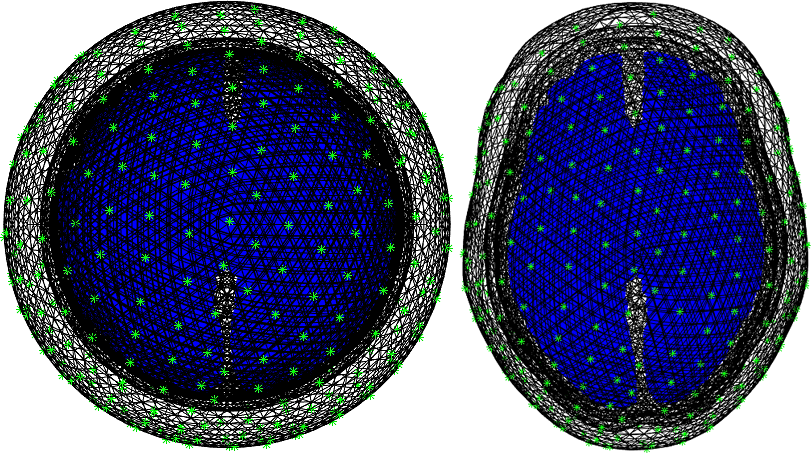
\includegraphics[width=1.0\textwidth]{casti/teorie/modely.png}
\caption{3-Shell Sphere a BEM modely hlavy}
\label{3-shell-sphere}
\end{figure}

Zjištění přesného rozložení jednotlivých hranic tkání mozku z MRI snímku je složitým problémem kvůli nízkým rozdílům kontrastů různých tkání. Záleží také na vážení MRI snímku (T1, T2 nebo protondensitní) \cite{24}. SPM12 využívá Forwinv toolboxu, který tento problém řeší s využitím standardního MNI mozku, který je geometricky transformován tak, aby výsledný model mozku vypadal jako ten z MRI snímků. Tento krok se nazývá prostorová normalizace (spatial normalization). Standardní MNI (Montreal Neurological Institute) mozek je vzorový model mozku, reprezentující normální populaci. Je průměrem 305 MRI snímků hlav zdravých lidí \cite{69}. Model hlavy, odvozený čistě z MRI nebo CT snímků, nikdy nebude stoprocentně shodný s modelem vypočteným pomocí prostorové normalizace. Odlišnost modelů však není natolik výrazná, aby byly výsledky inverzní úlohy jakkoli ovlivněny \cite{24}.

Vodivosti jednotlivých tkání jsou převzaté z literatury, z článků \cite{26} \cite{27} a~\cite{21}. Tkáně jsou považovány za čistě odporové, kapacitní a indukční efekty jsou zanedbány. Impedance tkání jsou tedy považovány za frekvenčně nezávislé. \cite{22} 

Přímá úloha také vymezuje oblasti, ve kterých se mohou zdroje aktivity nacházet. Zamezuje tak řešením, kdy by se zdroj aktivity mohl objevit mimo hlavu (takové řešení by teoreticky mohlo lépe odpovídat naměřeným datům, než jiná řešení). \cite{29}

\subsubsection{Měření pozic elektrod}
Digitalizace pozic senzorů se provádí takzvaným digitizérem. Jedná se o~systém, skládající se z ukazovátka a kamerového systému. Ukazovátko je vybavené orientačními body. Jeho špička se umístí na pozici měřené elektrody a~kamerový systém zaznamená pozice orientačních bodů. Ze znalosti pozic orientačních bodů a rozměrů ukazovátka je vypočtena pozice měřené elektrody v~prostoru.

Aby bylo zamezeno chybám, spojeným s případy, kdy se pacient během měření pohne a znehodnotí tak dosavadní měření, další orientační body jsou umístěny přímo na pacientově hlavě. Můžeme tak vždy zjistit polohu elektrody ve vztahu k aktuálnímu natočení a pozici pacientovy hlavy.

Během tohoto procesu je možné také nasnímat body, popisující tvar hlavy (headshape body), body na pacientově skalpu a obličeji. Tyto body jsou využívány pro zlepšení tvaru modelu pacientova mozku nebo pro zpřesnění koregistrace.

\subsubsection{Koregistrace}
Abychom byli schopni definovat řešení inverzní úlohy v MRI snímku pacientova mozku, potřebujeme znát pozice elektrod na pacientově skalpu, musíme provést sjednocení souřadnicových systémů MRI snímku a prostoru elektrod. Tento krok se nazývá koregistrace.
 
Souřadnicové systémy jsou sjednoceny výpočtem translačních a rotačních transformací prostorů. Parametry transformací jsou obvykle získány díky změření pozic tří orientačních bodů na pacientově lebce, jejichž polohu známe také v prostoru MRI snímku. Body jsou označovány jako fiducials. Nejčastěji používané fiducials jsou nasion a levý a pravý pre aurikulární bod, tedy kořen nosu a bod na levém a pravém uchu. \cite{29}

I když jsou pre-aurikulární body používané nejčastěji, je těžké tyto body lokalizovat přesně. Chyba v lokalizaci bodů vede k chybám v koregistraci (elektrody se mohou po transformaci nacházet například nad skalpem modelu), což ovlivňuje správnost inverzní úlohy. SPM12 toolbox řeší tento problém tak, že nejdříve napočítá transformaci z bodů fiducials a poté je koregistrace zpřesněna pomocí bodů, o kterých víme, že se nacházejí na skalpu pacienta. Mezi tyto body patří pozice elektrod, je ale možné využít headshape bodů. Počáteční transformace je zpřesněna metodou nejmenších čtverců. Nejlepší transformace minimalizuje sumu druhých mocnin vzdáleností bodů (pozic elektrod a headshape bodů) a skalpu.

Obecně je možné použít pro koregistraci jakékoliv tři body, známé v~obou souřadných systémech, je tedy možné využít například pozic některých elektrod, pokud známe jejich pozice v prostoru MRI. V takovém případě doporučuji volit body co nejvíce vzdálené od sebe, nepřesnost lokalizace vzdálených bodů vede k menší chybě koregistrace.

\begin{figure}[!h]
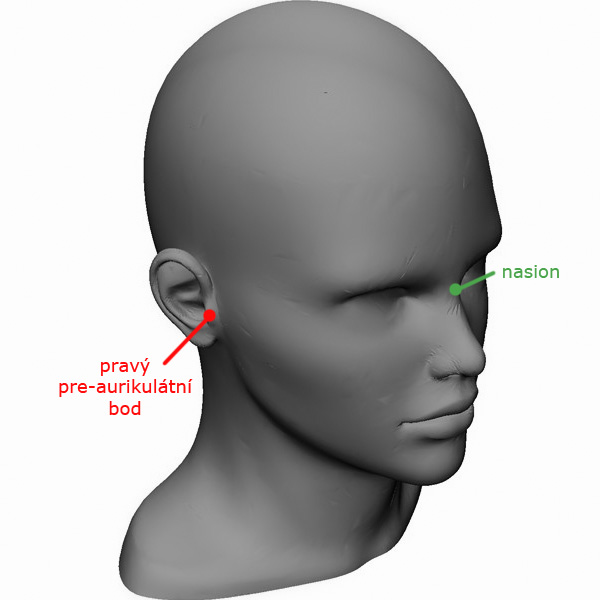
\includegraphics[scale=0.32]{casti/teorie/Fiducials.jpg}
\caption{Pozice bodů fiducials}
\end{figure}

\subsection{Inverzní úloha}
Lokalizace aktivní části mozku při dané mentální úloze je primárním záměrem zobrazovacích metod, zaměřených na centrální nervovou soustavu. Velká část výzkumu se zabývá zobrazováním pomocí PET (pozitronová emisní tomografie) a fMRI (funkční magnetická rezonance)\cite{30}. Tyto metody však nejsou ideální, pokud je otázkou, ve kterém časovém okamžiku během mentální úlohy byly jednotlivé části mozku aktivní. Pro řešení takového případu je nutné používat metody, které měří mozkovou aktivitu přímo, tedy elektroencefalografii nebo magnetoencefalografii. M/EEG signály nepřináší přímé důkazy o~umístění zdrojů aktivit. Jediný způsob, jak lokalizovat zdroje, je výpočtem inverzního problému. Inverzní úlohu lze vyřešit pouze pokud zavedeme předpoklady, které definují, jakým způsobem jsou M/EEG signály generovány. \cite{29} 

\subsubsection{Volba inverzní úlohy}
Obecně se algoritmy, řešící inverzní úlohu, snaží najít takové intrakraniální zdroje, které vytvářejí potenciály, shodné s potenciály naměřenými na skalpu pacienta. Základním problémem je však víceznačnost řešení. Naměřené skalpové potenciály lze obecně vysvětlit nekonečným množstvím konfigurací intrakraniálních zdrojů. Abychom byli schopni vyřešit takovou úlohu jednoznačně, je potřeba zavést předpoklady o zdrojích a vodivostech jednotlivých tkání. \cite{40,29}

\paragraph{Přeurčené modely}
Tyto metody inverze staví na dvou hypotézách: 

\begin{itemize}
\item Naměřený M/EEG signál se snaží vysvětlit pouze malým počtem proudových dipólů. 
\item Tyto dipóly jsou velmi fokální. 
\end{itemize}

Aby bylo dosaženo jednoznačného řešení, počet odhadovaných parametrů dipólů (každý dipól je popsán 6 parametry, 3 pro pozici, 2 pro natočení a 1 pro amplitudu) musí být nižší nebo roven počtu nezávislých měření (tedy počtu elektrod). Z procházeného stavového prostoru jsou postupně vybírány dipóly, pomocí nichž jsou vypočteny potenciálové mapy, které jsou následně porovnány s naměřenými potenciálovými mapami. Optimální řešení je zvoleno metodou nejmenších čtverců. Takové řešení minimalizuje součet čtverců rozdílů. Kvůli časové náročnosti výpočtů není možné projít stavový prostor celý, proto se přistupuje k optimalizačním procedurám, u kterých ale existuje risk uváznutí v lokálním optimu. Výpočetní nároky také rostou s~počtem hledaných dipólů, proto se typicky nepoužívá maximální možný počet dipólů daný měřením. \cite{28,29}

Přeurčené modely se snaží vytvořit model podle předpisu:
\begin{equation}
Y = L\vec{j} + e
\end{equation}

Kde $L=f(\vec{r})$ je transformační matice, $\vec{j}$ je orientace dipólů a $\vec{r}$ označuje polohu dipólů. Veličina $e$ označuje šum, který se objevuje v datech. Rovnice je řešena ve smyslu nejmenších čtverců. \cite{25}

Klíčovou otázkou zůstává, kolik aktivních zdrojů (tedy počet dipólů) se v~datech očekává. Tento parametr musí určit uživatel na základě svých zkušeností. Nejčastěji se počet volí na základě znalosti o tom, co data obsahují. Pro evokované potenciály nebo eliptické výboje se předpokládá velmi nízký počet aktivních zdrojů. Naopak aktivity, u kterých se očekává paralelní aktivace více míst, musí být popsány více dipóly. Existují také studie, navrhující metody, pro odhad početu dipólů na základě PET nebo fMRI. \cite{41,29}

Metoda lokalizace proudových dipólů je užitečná pro svou schopnost reprezentovat pozorovaná EEG data pomocí malého množství dobře interpretovatelných parametrů. Popsání mozkové aktivity pomocí malého počtu zdrojů zjednodušuje analýzu konektivity mezi těmito zdroji (dynamické kauzální modelování). \cite{42}

Nelze mezi sebou porovnávat modely s různými počty odhadovaných dipólů pouze na základě odchylky pozorovaných a modelovaných dat, protože s rostoucím počtem dipólů přesněji modelujeme pozorovanou aktivitu. Je však možné porovnávat takové modely na základě parametrů věrohodnosti (likelihood), které berou v potaz komplexnost modelů. \cite{42}

V SPM12 toolboxu je takováto metoda naimplementována pod zkratkou VB-ECDs (Variational Bayes Equivalent Current Dipoles) podle článku \cite{42}. Oproti jiným inverzním metodám ECD také umožňuje nadefinovat apriorní pravděpodobnost výskytu zdrojů aktivity, která může být vystavěna na empirických znalostech nebo dřívějších pozorováních pacienta. Tato pravděpodobnost může rozřešit situace, kdy různé dipóly modelují EEG data stejně dobře a model neposkytuje dostatek důkazů ve prospěch jednoho z řešení. \cite{28,42}

Existují přístupy optimalizace odhadu dipólů, takzvané „iterativní podmíněné režimy“ (ICM, iterative conditional mode). Je však známo, že tyto techniky nejsou invariantní a také nepočítají likelihood modelu \cite{42}. Tento optimalizační přístup je vhodný pro neinformované metody, kdy není definována apriorní pravděpodobnost, protože postup umožňuje projití lokálních maxim účelové funkce a nalezení dobrého výsledku. \cite{28}

\paragraph{Nedourčené modely}
Tyto metody jsou vhodné v případech, kdy počet dipólů není znám a nelze jej určit. Nedodurčené modely rekonstruují mozkovou aktivitu v každém bodě modelu pomocí tisíců dipólů fixní orientace rovnoměrně rozmístěných v modelu hlavy. Snahou je nalézt takovou unikátní konfiguraci zdrojových bodů, které co nejlépe odpovídají naměřeným datům. Problémem je to, že konfigurací zdrojových bodů, které přesně odpovídají naměřeným datům, je nekonečně velké množství. To znamená, že takový inverzní problém je nedostatečně podmíněný. Je tedy nutné přistoupit na další předpoklady, abychom byli schopni vybrat nejlepší řešení. V literatuře je navrženo mnoho různých omezení, která vedou k dobrým řešením. Některá jsou matematická, některá staví na znalostech fyziologie a některá vycházejí ze závěrů dalších zobrazovacích metod. Správnost těchto omezení je klíčová pro validitu řešení inverzního problému. \cite{29}

Nedourčený model je založený na lineárním mapování mezi dipólovými momenty fixního počtu dipólů a souborem signálů naměřených EEG nebo MEG. Tento vztah je dán vzorcem: 
\begin{equation}
Y = LJ + e
\end{equation}

Kde $Y$ je datový set M/EEG:
\begin{equation*}
Y \in {\rm I\!R}^{N_c \times N_n}
\end{equation*}

$N_c$ je počet senzorů a $N_n$ je počet časových vzorků, $J$ označuje neurální aktivitu zdrojů:
\begin{equation*}
J \in {\rm I\!R}^{N_d \times N_n}
\end{equation*}

$N_d$ je počet proudových dipólů distribuovaných modelem hlavy. Ty mají fixní orientaci kolmou k povrchu hlavy. Tyto dva sety jsou spojeny lead field matrix $L$:
\begin{equation*}
L \in {\rm I\!R}^{N_c \times N_d}
\end{equation*}

Měření je zatíženo Gaussovským šumem $e$ s nulovou střední hodnotou a~kovarianční maticí $Q_e$. Protože pro nedourčené modely obecně platí, že $N_d >> N_c$, pak nelze provést inverzi matice $L$ a tedy odhad $J$ nelze provést přímo. Za předpokladu, že $J$ má nulovou střední hodnotu a kovarianční matici $Q$, Bayesovská statistika umožňuje vytvořit odhad $\hat{J} = E[p(J|Y)]$, kde:
\begin{equation}
p(J|Y) = \frac{p(Y|J)p(J)}{p(Y)}
\end{equation}

Přičemž $p(Y)$ uvažovat nemusíme, protože je pro daná data konstantní a~vztah se nám zjednoduší:
\begin{equation}
p(J|Y) = p(Y|J)p(J)
\end{equation}

Jinými slovy se snažíme získat proudové rozložení $J$ založení na datovém souboru $Y$, kde $p(J)$ je stanovisko o zdrojích aktivity, které jsme stanovili ještě před měřením dat. Věrohodnost $p(Y|J)$ určuje pravděpodobnost, že dané proudové dipóly generují taková EEG data. $p(Y|J)$ má Gaussovské rozdělení $\mathcal{N}(LJ,Q_e)$. Protože $p(Y|J)$ i $p(J)$ mají normální rozdělení, můžeme psát:
\begin{equation}
p(Y|J)p(J) \propto \Theta = exp(-\frac{1}{2} (LJ-Y)^T Q^{-1}_e (LJ-Y)-\frac{1}{2}J^T Q^{-1} J)
\end{equation}

Optimální hodnoty aktivity zdrojů minimalizují $\Theta$, což odpovídá takové aktivitě, jejíž gradient $log(\Theta)$ je nulový:
\begin{equation}
\frac{d(log(\Theta))}{dJ} \Bigg\vert_{J = \hat{J}} = 0 = -L^T Q^{-1}_e (L\hat{J}-Y) - Q^{-1} \hat{J} 
\end{equation}

Z čehož je možné vyjádřit $\hat{J}$:
\begin{equation}
\hat{J} = Q L^T (Q_e + LQL^T)^{-1} Y
\label{vyslednaRovnice}
\end{equation}

Protože data $Y$ jsou známá a transformační matici $L$ lze vypočítat z modelu hlavy, potřebujeme pouze odhadnout kovarianční matice a jsme schopni získat zdrojové proudy $J$ v jediném algebraickém kroku.

Přesnost výpočtu velmi záleží na přesnosti, se kterou jsme schopni určit $Q$ a~$Q_e$. Předpokládáme, že kovarianční matice šumu senzorů má tvar:
\begin{equation*}
Q_e=h_0 I_{N_c}
\end{equation*}
Kde $I_{N_c}$ je jednotková matice o rozměru $N_c$ a $h_0$ je rozptyl šumu senzorů. \cite{74}

V následujících kapitolách si ukážeme několik příkladů omezení pro výběr řešení, nelze však pokrýt všechny algoritmy, protože jich je nesčetné množství. Nové algoritmy často vznikají jen drobnými úpravami již existujících algoritmů.





\paragraph{Minimum norm - MN}
\label{minimumNorm}
Minimum norm je obecným odhadem distribuce zdrojů v mozku a je počítáno bez jakékoliv apriorní informace \cite{43}. Tato metoda předpokládá pouze to, že nejlepší rozdělení proudových dipólů by mělo být takové, které má nejnižší intenzitu (minimalizuje Eukleidovskou normu). Z tohoto předpokladu plyne pouze jedno unikátní řešení, protože pouze jedna kombinace proudových dipólů stoprocentně modeluje pozorovanou mozkovou aktivitu a zároveň má nejnižší intenzitu. Předpoklad této metody o~celkové intenzitě však nemusí být fyziologicky správný. Tento algoritmus má v povaze znevýhodňovat taková řešení, která obsahují silné aktivace ložisek a dá tak přednost slabým a lokalizovaným aktivačním vzorům. Algoritmus MN také preferuje zdroje, nacházející se na povrchu mozku, protože takové zdroje vysvětlují pozorované EEG pomocí nižších amplitud proudových dipólů a~vedou na nižší Eukleidovskou normu. Zdroje, uložené hlouběji, jsou tedy nesprávně interpretovány jako jejich povrchové projekce.  \cite{29} 

Co se odhadu kovarianční matice týče, minimum norm algoritmus předpokládá, že \cite{74}:
\begin{equation}
Q = h_0 I_{N_d}
\end{equation}

Tato metoda inverze je v SPM12 toolboxu naimplementována pod zkratkou IID.

\paragraph{Weighted minimum norm - WMN}
Pro kompenzování tendence MN preferovat zdroje v blízkosti povrchu mozku, byla vyvinuta metoda Weighted minimum norm (WMN). Tento algoritmus přiřazuje povrchovým zdrojům nižší váhu, čímž umožňuje zdrojům uloženým hlouběji, aby byly vybrány jako výsledné řešení. Bylo vyvinuto několik strategií, jak určit váhy jednotlivých proudových dipólů, čímž vznikly algoritmy jako PROMS (Probabilistic reconstruction of multiple souces) \cite{44}, FOCUSS (Focal undetermined system solution) \cite{45} nebo RWMN (Radial weighted MN) \cite{46}.

\paragraph{Laplacian weighted minimum norm - LORETA}
Algoritmus LORETA přidává k WMN navíc další omezení a vybírá řešení s hladkým prostorovým rozložením, čehož dosahuje minimalizací Laplaciánu vážených řešení. Laplacián zde představuje míru prostorové drsnosti. Základem tohoto omezení je fyziologická úvaha, že aktivita neuronů v těsném sousedství je vzájemně korelovaná. I když je tento předpoklad v základu správný, existují kritiky zmiňující, že kvůli vzdálenosti bodů řešení a omezenému prostorovému rozlišení již není možné takové korelace očekávat. Vzhledem k tomu, že dvě funkčně rozdílná centra mohou být anatomicky velmi blízko sebe, což tento algoritmus nebere v potaz, je potřeba interpretovat výsledky metody s~opatrností. \cite{47,29}

V SPM12 toolboxu je velmi podobný algoritmus naimplementován pod zkratkou COH, jehož základem je MN algoritmus, ale bere také v potaz možnost korelace zdrojů do vzdálenosti několika milimetrů. \cite{28}

\paragraph{Multiple sparse priors – MSP}
MSP postupně prochází kombinace zdrojů a jejich konfigurace do té doby, dokud se zlepšuje shoda s pozorovanými daty \cite{28}. Měřítkem shody je v tomto případě logaritmická věrohodnost modelu.

Toto řešení inverzní úlohy staví na ReML (Restricted maximum likelihood) algoritmu, což je algoritmus, využívající log-likelihood kovariance hyperparametrů $\lambda$ (v Baysovské statistice apriorní parametry rozdělení) modelu $m$ a naměřených dat $Y$. Optimalizační kritérium lze formálně zapsat jako $ln(p(Y|\lambda,m))$. Problém MSP je podrobně popsán v \cite{51}. Optimalizace pomocí ReML algoritmu odstraní redundantní zdroje; jsou odstraněny takové zdroje, které jen málo přispívají ke zlepšení modelu. Zdroje aktivity jsou následně určeny pomocí ARD algoritmů (automatic relevance determination), které maximalizují shodu modulu a naměřených dat. \cite{52}

MSP je také možné vyjádřit jako pokračování rovnice \ref{vyslednaRovnice}, pomocí úvahy, že se kovarianční matice může skládat z váženého součtu více komponent $C = \{C_1, ..., C_N\}$, každé $C_i \in {\rm I\!R}^{N_d \times N_d}$:
\begin{equation}
Q = \sum\limits_{i=1}^N h_i C_i 
\end{equation}
$h = \{h_1, ..., h_N\}$ je vektor hyperparametrů váhujících kovarianční komponenty. \cite{74}

MSP algoritmus je optimalizován tak, aby vrátil co nejjednodušší rozložení zdrojů, kterými bude vysvětlovat většinu neměřených dat. \cite{28}

\paragraph{Greedy search – GS}
Greedy search je jednou z možností optimalizace algoritmu MSP. Vychází ze stejné kovarianční matice jako MSP, ale nejlepší konfiguraci hyperparametrů hledá iterativním prořezáváním sloupců kovarianční matice Q, které nedostatečně přispívají k nalezení dobrého řešení. \cite{74}

\paragraph{Beamformer}
Metoda Beamformer nebo také spatial filter (prostorový filtr) filtruje signál z elektrod takovým způsobem, že zachovávajá signál pouze ze zdroje aktuálního zájmu, ostatní signály jsou odfiltrovány \cite{20}. Metoda může být interpretována jako skenovací procedura, která dokáže odhadnout změny každého voxelu v čase. O prostorovém filtru můžeme smýšlet jako o virtuální elektrodě, kterou snímáme signál v daném voxelu. Touto elektrodou poté můžeme systematicky skenovat voxely v kterékoli části mozku a porovnávat jednotlivé aktivity \cite{49}. Oproti MN algoritmu a algoritmům z MN vycházejícím nemá Beamformer tendenci posouvat zdroje signálu blíže k povrchu hlavy \cite{46}. U této metody může docházet k potlačování některých zdrojů, pokud jsou takové dva zdroje oddělené a kovariantní. Bylo však dokázáno, že aby k~tomuto potlačení došlo, korelace zdrojů musí být celkem vysoká, vyšší než 0,7. \cite{50}

V toolboxu SPM12 je Beamformer naimplementován pod zkratkou EBB (Emirical Bayes Beamformer). Bayesovský je proto, že umožňuje nadefinovat apriorní pravděpodobnost výskytu zdroje aktivity na základě empirických znalostí, čímž je možné zpřesnit výsledek inverzní úlohy.

\subsubsection{Hodnocení výsledků inverzní úlohy}
Protože existuje velké množství algoritmů pro výpočet inverzního problému, vyvstává otázka, který z dostupných algoritmů zvolit a výsledky kterého algoritmu budou nejpřesnější. I když se jedná o rozhodující kritérium, neexistuje na takovou otázku jednoznačná odpověď, neboť neexistují metody, jak s jistotou určit zdroj aktivity. Není tedy výsledky inverzní úlohy s čím porovnat. To je také důvodem, proč neexistuje zlatý používaný standard. \cite{29}

Jednou z používaných metod, jak výsledky ověřit, je výpočet inverzní úlohy na syntetických datech, o kterých s jistotou víme, kde mají v mozku zdroj aktivity. Syntetická data jsou vytvořena pomocí přímé úlohy, která má za úkol modelovat pacientovu hlavu. Do modelu hlavy je umístěn proudový dipól a následně jsou vypočteny a uloženy potenciály, které tento dipól vyvolá na skalpu modelu. Chyba inverzní úlohy je určena jako rozdíl mezi pozicemi odhadnutého a skutečného ložiska aktivity. Tento přístup byl v minulosti použit ke zkoumání závislosti chyb algoritmů inverzních úloh na pozici ložiska \cite{54}, ke zkoumání závislosti chyb algoritmů inverzní úlohy na hloubce, ve které bylo ložisko aktivity uloženo \cite{55}, k určení vlivu šumu na výsledky inverzní úlohy \cite{23} nebo k určení vlivu typu modelu hlavy na výsledky inverzní úlohy \cite{56}.


\section{Somatosenzorické evokované potenciály}

Somatosenzorické evokované potenciály na nervus medianus vyvolávají odpověď v kontralaterální hemisféře v primární senzitivní korové oblasti pro ruku. To znamená, že SEPy levé ruky mají odezvu v pravé hemisféře v gyrus postcentralis, tedy v konvexitě, kde by měly být proudové dipóly dobře zachytitelné. V homunkulu je dobře znázorněno, kde na konvexitě aktivitu očekávat. Kvůli velké citlivosti horních končetin je aktivační oblast proporcionálně velká. \cite{68}

\begin{figure}[!h]
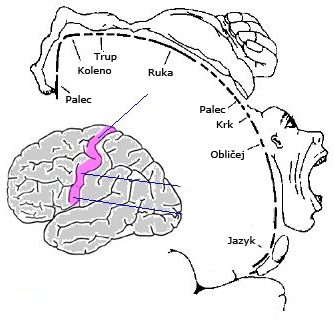
\includegraphics[scale=0.5]{casti/aplikace/sep/homunculus.jpg}
\caption{Homunkulus}
\end{figure}

Co se týče EEG signálu, hlavní složkou by měla být negativní vlna v dané oblasti, na kterou mohou navazovat další signály z okolních korových oblastí (z~primární i sekundární motorické oblasti a sekundární senzitivní oblasti), ty by ale měly mít nižší amplitudu. Vlna, kterou hledáme, by měla mít amplitudu přibližně 10~$\mu$V, její maximum se nachází asi po 19 ms po stimulačním impulsu (v závislosti na délce pacientovy paže se může čas maxima mírně lišit). \cite{68}

\begin{figure}[!h]
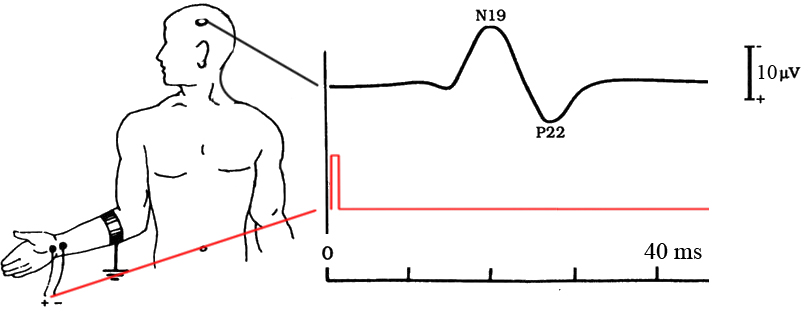
\includegraphics[scale=0.5]{casti/aplikace/sep/odezva.jpg}
\caption{Znázornění odezvy na stimul nervus medianus}
\end{figure}



%!TEX ROOT=../../Diplomka.tex

\chapter{Implementace}

\section{SPM Motol toolbox}
Vzhledem k faktu, že pro úspěšnou aplikaci výpočtu inverzní úlohy je potřeba provést velké množství přípravných procedur, které jsem naimplementoval do různých funkcí, řešil jsem otázku, jak dostat balík těchto funkcí k lidem, kteří budou metody využívat. Rozhodl jsem se vytvořit SPM Motol toolbox, který obsahuje SPM12 toolbox, upravuje některé jeho funkce a přikládá mnou implementované funkce. Jedná se tedy o rozšíření SPM12 toolboxu. Mezi podstatnou úpravu původního SPM12 toolboxu patří možnost generovat výsledky inverzní úlohy do MRI snímků našich pacientů, namísto do standardního MNI mozku. Přiložené funkce a jejich možnosti si projdeme v~následujících kapitolách.


\subsection{Instalace}
Pro snadné vložení SPM Motol toolboxu do prostředí Matlabu jsem vytvořil \textbf{SPM12Motol\_Installer.m}. Jedná se o instalační skript pro operační systém Windows, který stačí spustit v prostředí Matlab a provede automatické zkopírování toolboxu do složky s ostatními toolboxy a přidá potřebné cesty, díky kterým bude Matlab moci využívat funkce toolboxu v dalších skriptech.

Úspěšnost dokončení instalace lze ověřit pomocí příkazu \textbf{testing\_motol}. Pokud tento příkaz nevypíše chybovou hlášku, je toolbox nainstalován úspěšně.



\section{Předzpracování dat}
Techniky předzpracování dat, neboli preprocessing, jsou procedury nad daty, které připravují data pro další kroky zpracování. Upravují data pro jednodušší nebo efektivnější aplikaci dalších procedur. Nevhodné nebo nedostatečné předzpracování by mohlo vést k zavádějícím výsledkům.

\subsection{Notch filtr}
Notch filtr je filtr typu pásmová zádrž, který se používá k odfiltrování velmi úzké části frekvenčního pásma. Typicky jsou jím filtrovány rušivé signály naindukované na vodiče, které se vždy nacházejí na konkrétním úzkém pásmu frekvence a ovlivňují měření. V podmínkách České republiky jde hlavně o~síťové rušení na kmitočtu 50 Hz (v Americe by se jednalo o 60 Hz).

Skalpové EEG signály jsou velmi slabá napětí v rozsahu od 2 do 200~$\mu$V a~typicky jsou měřena za přítomnosti síťového rušení. Ačkoli je možné zavést opatření, která sníží hladinu síťového rušení, jeho indukci nelze nezabránít úplně. Síťové rušení se může na některých elektrodách projevovat znatelněji než na jiných. Odfiltrování frekvence síťového rušení je tedy nutností. \cite{63}

Pro návrh notch filtru jsem využil membránového konceptu, ze kterého vyplývá, kde musí být umístěny nuly (kořeny čitatele přenosové funkce) filtru v modulu přenosové funkce v z-rovině. První nula musí být umístěna na jednotkové kružnici pod takovým úhlem, který odpovídá frekvenci, kterou chceme odstranit. Druhá nula je poté komplexně sdružená s první. První pól (kořen jmenovatele přenosové funkce) leží v jednotkové kružnici pod stejným úhlem jako první nula. Vzdálenost pólu a příslušné nuly ovlivňuje šířku frekvenčního pásma, které bude filtrem odstraněno. Argument, ovlivňující tuto šířku, bude součástí navrhované funkce. Druhý pól je opět komplexně sdružený prvnímu pólu. \cite{64}

Navrhl jsem Matlab funkci \textbf{Notch}, jejímž vstupem jsou tři argumenty: vzorkovací frekvence, pro kterou filtr navrhujme, frekvence, kterou chceme odstranit a~parametr B, ovlivňující šířku pásma. Výstupem funkce jsou koeficienty čitatele a jmenovatele přenosové funkce filtru.
\begin{figure}[!h]
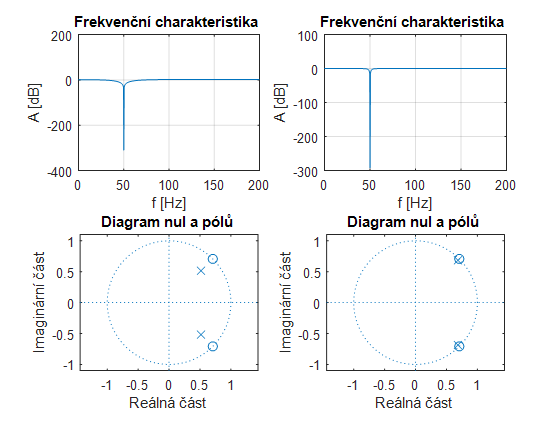
\includegraphics[width=1.0\textwidth]{casti/implementace/notch/charakteristika.png}
\caption{Charakteristiky notch filtrů 50 Hz}
\end{figure}

\newpage
Filtry byly navrženy pro vzorkovací frekvenci 400 Hz, levý sloupec je vykreslen pro šířku pásma 20 Hz, pravý sloupec je vykreslen pro šířku pásma 2 Hz.

\begin{figure}[!h]
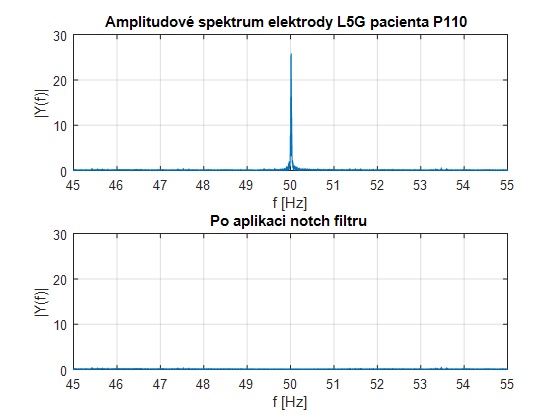
\includegraphics[width=1.0\textwidth]{casti/implementace/notch/aplikace.png}
\caption{Frekvenční spektra reálného EEG signálu před a po aplikaci filtrace notch filtrem}
\label{aplikacedrift}
\end{figure}

V obrázku \ref{aplikacedrift} byl použit notch filtr, navržený pro vzorkovací frekvenci 2048~Hz, zádrž 50~Hz, šířka pásma 1~Hz.

Pro jednoduchou aplikaci jsem připravil funkci \textbf{ApplyNotch}, která automaticky aplikuje filtraci na celý datový soubor. Vstupními argumenty jsou matice dat, jejich vzorkovací frekvence a frekvence, která bude odfiltrována.


\subsection{Odstranění izolinie}
Kolísání izolinie neboli drift je jev, zkreslující naměřená data a objevující se nejen u EEG, ale i u dalších signálů, které je možné na pacientech měřit. Protože se spektra driftu a užitečného signálu překrývají, snažíme se najít takovou metodu, která spektrum užitečného signálu ovlivní nejméně. Kolísání izolinie je způsobeno elektrochemickými ději na rozhraní kůže a elektrody, které jsou následkem nedokonalého kontaktu elektrody a pohyby pacienta. Rušení má náhodný charakter a pro jeho odstranění se používá horní propusť s mezní frekvencí 0,5 Hz. \cite{65,66}

Literatura doporučuje odstranění izolinie pomocí 0,5 Hz hornofrekvenční propusti, při vzorkovací frekvenci 2048 Hz, kterou jsou naměřena EEG data v nemocnici Motol, takový filtr dosahuje nepraktického množství koeficientů. Za použití funkce fir1 pro návrh filtru, přechodové pásmo 0,35 až 0,65 Hz, potlačení 0 dB v propustné části a -40 dB v nepropustné části, dosahuje filtr délky 15 241 koeficientů. Velké množství dat v kombinaci s využitím filtrační funkce filtfilt (filtruje signál dvakrát, od začátku do konce a poté od konce k~začátku, čímž dosahuje nulového zpoždění v signálu), jsou výpočetní nároky příliš vysoké. Pro snížení délky filtru se nabízí možnost decimace signálu, ta ale vyžaduje odstranění aliasing efektu dolní propustí. Pokud bych po odstranění izolinie signál opět interpoloval na původní kmitočet, výsledkem by byl pozměněný signál.

Rozhodl jsem se tedy provést odstranění izolinie jejím odhadem pomocí 0,5 Hz dolní propusti a následným odečtením izolinie od původních dat. Rozdílem od původního přístupu je možnost decimace signálu, aniž bych ovlivnil výsledné spektrum užitečného signálu, čímž dosáhnu kratšího filtru. Signál decimuji faktorem 100, operaci jsem rozložil do dvou decimací faktory 10. Vyšší frekvence, které by mohly být zkresleny aliasingem, budou odfiltrovány aplikací 0,5 Hz dolní propustí. Pro návrh tohoto filtru jsem použil funkce fir1, s přechodovým pásmem 0,35 až 0,65 Hz, potlačením 0 dB v propustné části a -40 dB v nepropustné části. Výsledný filtr má nyní délku pouhých 154 koeficientů a filtrace stejných dat funkcí filtfilt se oproti původnímu přístupu zrychlila cca 75-krát (může se mírně různit v závislosti na vytížení počítače). Aplikací filtrace získám odhad driftu, který lineárně interpoluji na původní frekvenci a odečtu od původních dat.

Celý proces jsem naimplementoval do Matlab funkce \textbf{deleteDrift}. Vstupem funkce je matice s naměřenými EEG daty a vzorkovací frekvence, výstupem jsou EEG data s odstraněným driftem.

\begin{figure}[!h]
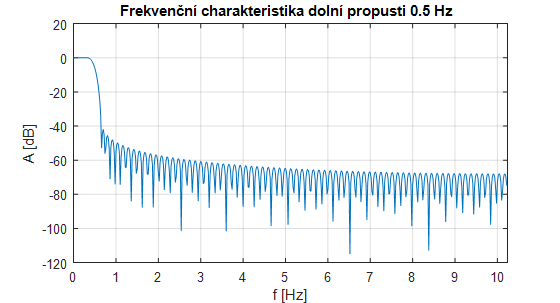
\includegraphics[width=1.0\textwidth]{casti/implementace/izolinie/charakteristika.png}
\caption{Frekvenční charakteristika dolní propusti o mezní frekvenci 0,5 Hz navržená funkcí fir1}
\end{figure}

\begin{figure}[!h]
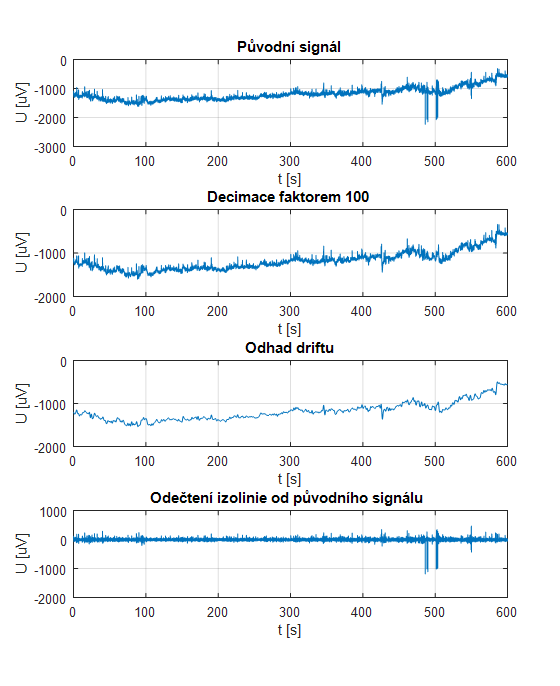
\includegraphics[width=1.0\textwidth]{casti/implementace/izolinie/aplikace.png}
\caption{Proces odstranění izolinie z dat}
\end{figure}

\subsection{Oprava zesilovačů}
Data, naměřená v nemocnici Motol, jsou měřena pomocí sytému firmy ANT Neuro, dnes již nedostupným modelem Asa lab. Tento systém je sice 256-kanálový, ale je složen ze dvou zesilovačů, přičemž každému z nich náleží 128 elektrod. Oba zesilovače měří v referenčním zapojení s průměrnou referencí. U některých pacientů se stalo, že se jednotlivé reference výrazně lišily a hodnoty na elektrodách jednoho zesilovače několikanásobně převyšovaly hodnoty zesilovače druhého. V takovém případě pak inverzní úloha dává nesmyslné výsledky, protože aktivita se nutně objeví pod pozicemi elektrod s vysokými hodnotami.

\begin{figure}[!h]
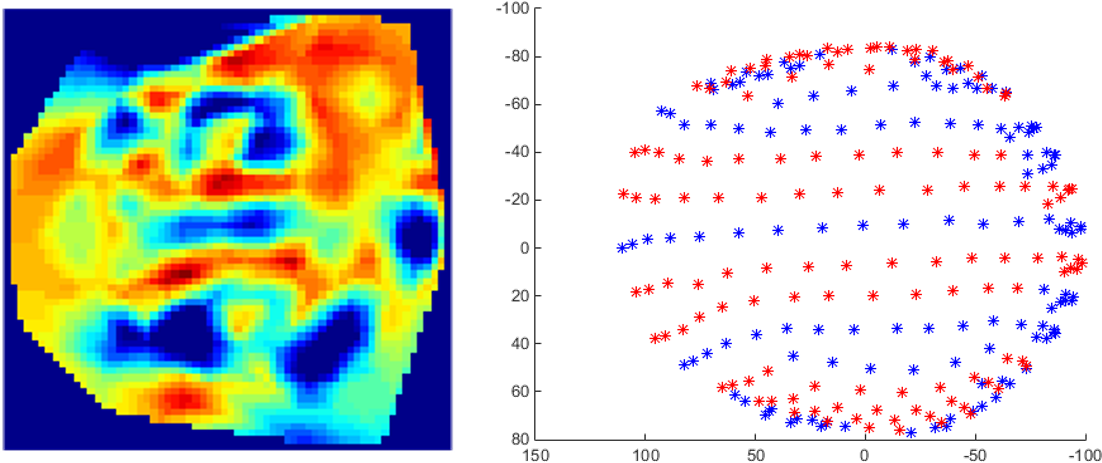
\includegraphics[width=1.0\textwidth]{casti/implementace/opravazesilovacu.png}
\caption{Potenciálová mapa skalpu pacienta, elektrody na skalpu pacienta}
\label{opravazesilovacu}
\end{figure}

Na obrázku \ref{opravazesilovacu} je vidět, že pod modrými elektrodami se vyskytují potenciály s nízkými hodnotami. Červená a modrá barva odlišuje, kterému zesilovači elektroda přísluší.

Tento problém jsme vyřešili přereferencováním signálů obou zesilovačů. V~praxi to znamená, že z každého časového vzorku signálů elektrod jednoho zesilovače je vypočtena průměrná hodnota, která je následně odečtena od hodnot těchto kanálů v tomto časovém vzorku. Stejný postup je aplikován pro signály elektrod druhého zesilovače. Postup se opakuje pro všechny časové vzorky signálu.

Tento proces je naimplementován ve funkci \textbf{amplifierCorrection}, jejímž vstupem je matice dat a dva vektory, ve kterých se nacházejí indexy elektrod jednotlivých zesilovačů. Z těch je následně vypočítána nová reference.



\section{Pomocné funkce}
Kromě funkcí pro předzpracování dat jsem naimplementoval další funkce, které by se v budoucnosti mohly hodit obsluze inverzní úlohy.

\paragraph{Vykreslení pozic elektrod}
Vytvořil jsem funkci \textbf{plotHead}, jejímž vstupem jsou dva argumenty: cesta k~elc souboru, obsahující pozice elektrod a headshape bodů a cesta k elc souboru, který obsahuje body fiducials. Funkce vykreslí trojrozměrný otočný graf s pozicemi elektrod.

\begin{figure}[!h]
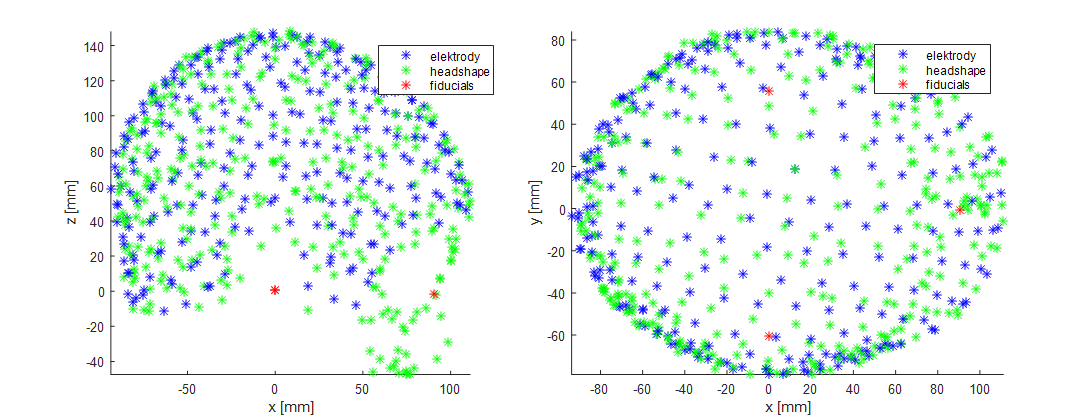
\includegraphics[width=1.0\textwidth]{casti/implementace/head/hlava.png}
\caption{Dvě různá natočení výstupního grafu funkce plotHead}
\end{figure}


\paragraph{Spektrum signálu}
Další užitečnou funkcí je vykreslení jednostranného spektra signálu. Funkce se jmenuje \textbf{signalSpectrum}. Jejím vstupem je cesta k souboru, který obsahuje EEG data, vzorkovací frekvence a vektor s indexy elektrod, jejichž spektrum chceme vykreslit.


\section{Inverzní úloha}
I když pro samotný výpočet inverzní úlohy využívám SPM12 toolbox, stále je potřeba vytvořit potřebné soubory, které budou definovat parametry inverze. Tyto soubory jsou vytvářeny pomocí informací obsažených v datech naměřených na pacientovi. Jejich tvorbu zajišťuje volání jediné funkce.

\subsection{Soubory, potřebné pro výpočet inverzní úlohy}
Prvním ze souborů, potřebných pro výpočet inverzní úlohy, jsou naměřená EEG data. Naměřená data mi jsou předávána v několika souborech Matlab formátu s koncovkou .mat. Rozdělená jsou lépe spravovatelná a umožňují zpracování jen souborů s událostmi, které nás aktuálně zajímají. Každý soubor obsahuje 5 minut EEG záznamů všech elektrod, vzorkovací frekvenci, kterou byla data naměřena, hlavičku, popisující data a vektor, obsahující časy jednotlivých vzorků EEG dat. Hlavička dat je uložena v proměnné header a~obsahuje položky popsané v následující tabulce:

\begin{table}[!h]
\begin{ctucolortab}
\begin{tabular}{lp{8.5cm}}
\bfseries Položka hlavičky & \bfseries Popis \\
\Midrule
header.label & 	Názvy jednotlivých elektrod \\
header.rate & 	Vzorkovací frekvence \\
header.npnt & 	Počet vzorků v datovém souboru \\
header.nchan & 	Počet kanálů datového souboru \\
header.time & 	Vektor časů jednotlivých vzorků EEG dat \\
header.triggers & 	Struktura, popisující události v datech, převážně používaná při měření evokovaných potenciálů \\
header.startdate & 	Datum a čas počátku měření EEG \\
header.triggers\_tabs & 	Časy jednotlivých událostí
\end{tabular}
\end{ctucolortab}
\caption{Popis hlavičky EEG dat}
\label{hlavickaEEG}
\end{table}

K výpočtu inverzního problému dále potřebujeme znát pozice elektrod na skalpu pacienta a pozice bodů fiducials, umožňující správnou koregistraci. Tyto informace jsou zakódovány v souborech s koncovkou .elc a body z nich jsou čteny pomocí funkcí \textbf{elc\_read} a \textbf{fiducials\_read}. Obě funkce mají jeden vstupní parametr, kterým je cesta k příslušnému souboru.

Posledním potřebným souborem je MRI snímek pacientovy hlavy v souboru formátu NIfTI. 

NIfTI (Neuroimaging Informatics Technology Initiative file format) je využíván mnoha softwary zabývajícími se metodami zobrazování, je náhradou za starší ANALYZE formát, který neobsahoval informace o orientaci snímku.
U~NIfTI formátu může také dojít k záměně orientace, uživatel si musí dát pozor, v~jaké rovině software vykresluje snímky.
K záměně levé a pravé strany hlavy může dojít, protože uživatel není schopen určit, ze kterého směru se na řez dívá, zda jde o pohled odspoda nahoru či obráceně. Některé softwary (jako například 3D Slicer) vykreslují snímky v RAS (Right-Anterior-Superior) rovině, kdy se pravá strana hlavy promítne na obrázku vlevo, jiné programy (příkladem je SPM) vykreslují do LPS (Left-Posterior-Superior) roviny.

MRI snímky jsem obvykle obdržel ve formátu Dicom (Digital Imaging and Communications in Medicine). Převedl jsem je na snímky formátu NIfTI pomocí softwaru MRIcron, který je připraven v balíku SPM Motol toolbox spolu s návodem k použití.


\subsection{Načtení EEG dat}
I když je rozdělení EEG dat do více souborů výhodné, pro aplikaci předzpracování je nutné soubory opět spojit do jednoho velkého celku. Pro tento účel jsem vytvořil funkci \textbf{loadEEGData}, jejímž vstupem je cesta ke složce, ve které jsou vybrané soubory pro zpracování uloženy. Metoda postupně načte jednotlivé soubory, jejich data seřadí za sebe a vytvoří jednu společnou hlavičku, popisující data jako celek. Výstup funkce je stejný, jako by byl načten jeden velký soubor s EEG daty.

\subsection{Selekce událostí}
Funkce \textbf{cutTrials}, kterou jsem naimplementoval, umožňuje selekci pouze těch událostí, které nás aktuálně zajímají.
Tato funkce bude použita např. v~případě, kdy se v aktuálně načteném souboru EEG dat somatosenzorických evokovaných potenciálů nacházejí stimulace levé i pravé končetiny. Tato funkce umožní vybrat evokované potenciály pouze jedné z končetin jednoduchým vložením indexů první a poslední události do argumentu funkce.

Funkce \textbf{generateSPMTrialsStruct} vzápětí vygeneruje strukturu, popisující události v datech. Tuto strukturu využijeme v následující funkci.


\subsection{Tvorba souboru kompatibilního s SPM12}
\label{tvorbaSPMsouboru}
Pro analýzu EEG signálu je potřeba převést data do formátu srozumitelného pro SPM12. SPM12 toolbox je schopen automaticky převádět data z různých formátů, jako je biosemi nebo biosig. Využívá k tomu toolboxu fileIO, který je schopen rozpoznat a převést data z většiny komerčních EEG zařízení. Data jsou automaticky převedena do dvou souborů *.dat a *.mat, kde .dat soubor je binární soubor, obsahující EEG záznam a .mat soubor obsahuje hlavičku s~popisem dat a odkazuje se na .dat soubor. Soubory, ve kterých dostáváme data, bohužel nepatří mezi automaticky převeditelné soubory, proto jsem naimplementoval vlastní konvertor. 

Z počátku jsem data převáděl do formátu .gdf. Tento formát je automaticky převoditelný pomocí SPM12 funkce Convert. Od převodu do .gdf jsem ale upustil, protože hlavička souborů tohoto formátu neumožňuje nadefinovat některé potřebné struktury, jako je například struktura popisující události nastalé v datech, nebo struktura popisující pozice elektrod.

Jako další řešení jsem zvolil tvorbu vlastní funkce, která bude převádět data přímo do formátu srozumitelného SPM12. Funkce se jmenuje \textbf{createSPMFile}. Funkce nejprve ověří, zda se shodují názvy elektrod s názvy kanálů v~datech. Pokud není některý kanál nalezen například z důvodu chyby v jeho označení, vypíše se varovná hláška. V dalším kroku je vytvořena proměnná jménem $D$, to je struktura obsahující všechny informace o datech i data samotná. Funkce automaticky vyplní pole hlavičky popsané v tabulkách 
\ref{SPMhlavicka1cast} a \ref{SPMhlavicka2cast}.

\begin{table}
\begin{ctucolortab}
\begin{tabular}{lp{8.5cm}}
\bfseries Položka hlavičky & \bfseries Popis \\
\Midrule
D.type & 	Typ dat: 'continuous', 'single' nebo 'evoked' \\
D.Nsamples & 	Počet vzorků dat \\
D.Fsample & 	Vzorkovací frekvence \\
D.timeOnset & 	Čas prvního vzorku \\
D.data & 	Matice s EEG daty \\
D.fname & 	Jméno souboru, který bude vytvořen \\
D.fpath & 	Cesta k vytvářenému souboru \\
D.trials & 	Celkový popis událostí \\
D.trials.label & 	Názvy nastalých událostí \\
D.trials.onset & 	Čas prvního vzorku první události \\
D.trials.bad & 	Příznak, poukazující na události nevhodné pro další zpracování \\
D.trials.repl & 	V případě průměrovaných dat popisuje, z kolika událostí byla data vytvořena \\
D.trials.events & 	Struktura, popisující události v datech, která byla předpřipravena funkcí generateSPMTrialsStruct \\
D.trials.events.type & 	Název popisované události \\
D.trials.events.value & 	Kódové číslo události \\
D.trials.events.time & 	Čas začátku události v sekundách \\
D.trials.events.duration & 	Doba trvání události \\
D.channels & 	Struktura, popisující kanály záznamu, musí odpovídat pořadí kanálů v datech \\
D.channels.label & 	Název kanálu \\
D.channels.type & 	Typ záznamu - 'MEG', 'EEG', 'VEOG', 'HEOG', 'EMG', 'LFP' \\
D.channels.units & 	Jednotky kanálem měřené veličiny  \\
D.channels.bad & 	Příznak, poukazující na kanál nevhodný pro další zpracování \\
D.channels.X\_plot2D & 	X souřadnice pozice na 2D ploše \\
D.channels.Y\_plot2D & 	Y souřadnice pozice na 2D ploše \\
D.sensors & 	Struktura, upřesňující informace o elektrodách \\
D.sensors.eeg.chanpos & 	Matice, obsahující pozice kanálu na skalpu \\
D.sensors.eeg.chantype & 	Typ záznamu - 'MEG', 'EEG', 'VEOG', 'HEOG', 'EMG' ,'LFP' \\
D.sensors.eeg.chanunit & 	Jednotky kanálů \\
D.sensors.eeg.elecpos & 	Matice, obsahující pozice elektrod na skalpu, totožná s D.sensors.eeg.chanpos \\
D.sensors.eeg.label & 	Názvy kanálů \\
D.sensors.eeg.type & 	Výrobce snímacího zařízení \\
D.sensors.eeg.unit & 	Jednotka souřadnic poloh elektrod
\end{tabular}
\end{ctucolortab}
\caption{Popis hlavičky SPM souboru 1. část}
\label{SPMhlavicka1cast}
\end{table}


\begin{table}
\begin{ctucolortab}
\begin{tabular}{lp{8.5cm}}
\bfseries Položka hlavičky & \bfseries Popis \\
\Midrule
D.fiducials & 	Struktura pro popis tvaru lebky pomocí headshape a fiducials bodů \\
D.fiducials.pnt & 	Matice, obsahující headshape body \\
D.fiducials.fid.pnt & 	Souřadnice tří fiducials bodů \\
D.fiducials.fid.label & 	Názvy těchto fiducials bodů \\
D.history & 	Struktura, uchovávající historii modifikací dat \\
D.history.function & 	Název operace volané na data \\
D.history.arguments & 	Argumenty funkce \\
D.history.time & 	Čas volání funkce \\
D.montage & 	Informace o použitých montážích \\
D.montage.M & 	Transformační matice, popisující operace s kanály a definice nových kanálů, umožňuje například odečítání dvou kanálů pro zisk bipolárního zapojení \\
D.montage.Mind & 	Indikuje, která transformační matice byla použita pro vytvoření dat
\end{tabular}
\end{ctucolortab}
\caption{Popis hlavičky SPM souboru 2. část}
\label{SPMhlavicka2cast}
\end{table}

Takto vytvořená struktura je následně uložena do souboru, který je nyní možné načíst pomocí SPM12 toolboxu a provádět nad ním další operace.

\subsection{Selekce oken a průměrování}
V EEG datech nás typicky zajímají ERP (event related potencials), to jsou malé časové úseky EEG okolo nastalých událostí (takzvaná okna). Proces selekce těchto oken se v SPM12 nazývá epoching. Během tohoto procesu jsou data mimo události odstraněna.

Události jsou jednak reakcí na stimul (evokované potenciály), kdy jsou časy událostí zaznamenány systémem, který vytváří stimuly. Druhou možností jsou události, nastávající náhodně (například komplexy hrot-vlna u epileptiků), jejichž přesné časové umístění dohledáváme pomocí detektorů typických grafoelementů. Ať už se jedná o první nebo druhý typ událostí, okna jsou vždy zatížena náhodnou aktivitou okolních neuronů, která s danou událostí nesouvisí. Proto se vždy snažíme nasbírat co největší množství událostí a~aplikovat metodu průměrování. Vytvořením průměru z oken získáme krátký časový úsek s~nízkou úrovní náhodné aktivity, na který je aplikován výpočet inverzní úlohy. 
Velikost náhodné složky klesá na násobek $\frac{1}{\sqrt{n}}$, kde n je počet realizací.
Náhodná složka by teoreticky byla zcela odstraněna, kdybychom měli k~dispozici nekonečné množství oken.
 
Proces selekce oken a průměrování je již naimplementován v SPM12 toolboxu. Musíme si však připravit pomocný soubor, ve kterém jsou nadefinována okna pro ořez dat. Soubor vytváří funkce s názvem \textbf{prepareTrialsFile}. Vstupem do ní jsou dva argumenty. Je to struktura popisující události, kterou generuje výše popsaná funkce \textbf{generateSPMTrialsStruct} a druhým argumentem je specifikace délky časového okna. Jedná se o vektor dvou časů v~milisekundách, popisující, jak dlouhý časový úsek okolo události bude zachován. Čas událostí je označen nulou, záporný čas označuje dění před událostí. Funkce vygeneruje potřebný soubor a uloží jej do aktuálního adresáře.

Aplikaci selekce oken a průměrování provedeme pomocí Batch editoru SPM12 toolboxu. Jedná se o nástroj, umožňující automatizovat operace nad datovými soubory. Z nabídky funkcí Batch editoru vybereme Preprocessing – Epoching a Averaging. Vstupem epochingu je soubor, obsahující EEG data (výstupní soubor kapitoly \ref{tvorbaSPMsouboru}) a soubor vygenerovaný v minulém kroku, který popisuje, jaká okna budou vybrána. Proces průměrování nastavíme jako závislý, čímž specifikujeme, že průměrování bude aplikováno na výstupní data kroku epoching. Spuštění těchto kroků je možné provést buď přímo v Batch editoru zelenou šipkou v~horní části grafického rozhraní, nebo je možné si vytvořený skript uložit do souboru a kroky spustit pomocí funkce spm\_jobman (soubor je vstupním argumentem), která je součástí SPM12 toolboxu.

\subsection{Výpočet inverzní úlohy}
Specifikaci a výpočet inverzní úlohy je možné v SPM12 toolboxu provést dvěma způsoby. Jedním je využití grafického rozhraní, které je vyvoláno stiskem tlačítka 3D Source Reconstruction. Druhou možností je využitím Batch editoru.

\subsubsection{3D Source Reconstruction}
Uživatelské rozhraní pro výpočet inverzního problému je intuitivní, aktivní jsou vždy jen ta tlačítka, kterými je nutné specifikovat aktuální krok. Výhodou rozhraní je možnost kontroly správnosti jednotlivých kroků, rychlá změna nastavení parametrů inverze a možnost grafického znázornění výsledků inverze v MRI snímcích.

Při prvním spuštění je aktivní pouze tlačítko Load, kterým načteme EEG datový soubor, se kterým budeme pracovat a do kterého se budou jednotlivé kroky ukládat. V druhém kroku specifikujeme model pacientovy hlavy. Máme možnost výběru mezi modelem standardního mozku nebo výpočtem modelu z pacientova MRI snímku. Výpočet modelu trvá několik minut, po dokončení výpočtu se zobrazí vypočtený model hlavy spolu s několika řezy MRI snímkem. Uživatel má tak možnost posoudit, zda byl model vypočten správně (příklad viz \ref{prikladMRImodelu}).

\begin{figure}[!h]
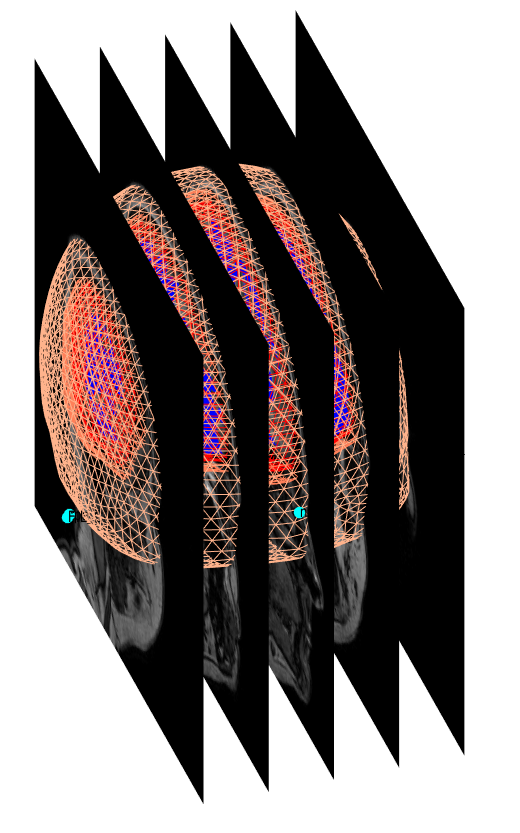
\includegraphics[width = 6cm]{casti/implementace/sourceReconstruction/MRI.png}
\caption{Model vypočtený z MRI snímků pacientovy hlavy}
\label{prikladMRImodelu}
\end{figure}

Následujícím krokem je koregistrace. Rozhraní provede uživatele specifikací bodů fiducials. Ty je možné specifikovat třemi způsoby: výběrem ze seznamu nadefinovaných fiducials, vepsáním souřadnic bodů nebo kliknutím do modelu myší, čímž uživatel určí přibližnou polohu bodů. Po dokončení transformací prostoru MRI a prostoru elektrod je vykreslen výsledek koregistrace, elektrody by měly přesně padnout na skalp modelu (viz \ref{prikladKoregistrace}).

\begin{figure}[!h]
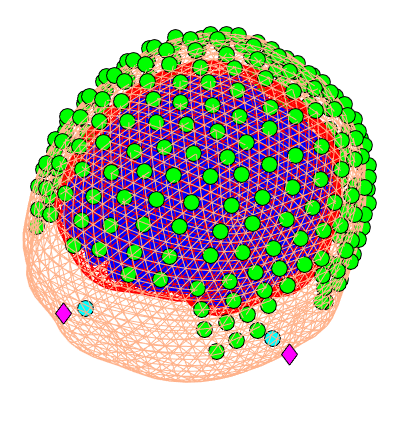
\includegraphics[width = 6cm]{casti/implementace/sourceReconstruction/Corregistration.png}
\caption{Výsledek koregistrace}
\label{prikladKoregistrace}
\end{figure}

Následně je zpřístupněno tlačítko Forward Model, kde dostaneme možnost výběru mezi dostupnými modely. Pro EEG data máme možnost výběru mezi 3-shell sphere nebo BEM modely (modely jsou popsány v kapitole \ref{primaUloha}). Vždy volím anatomicky přesnější a výpočetně náročnější BEM model. Po dokončení finálního výpočtu modelu je model naposledy zobrazen (obrázek viz \ref{3-shell-sphere}). Uživatel provede finální inspekci modelu. Pokud zjistí nesrovnalosti, může kterýkoli z kroků zopakovat a opravit. Dokončením tohoto kroku jsme úspěšně nadefinovali přímou úlohu a v grafickém rozhraní je zpřístupněna možnost výpočtu inverzní úlohy.

Proces výpočtu inverzní úlohy začíná volbou parametrů. Prvním je výběr mezi přeurčenými (tlačítko VB-ECD) nebo nedourčenými modely (tlačítko Imaging). Zvolím nedourčené modely, které jsou intuitivnější a podle mých zkušeností dávají na předložených datech lepší výsledky. Dále máme na výběr mezi dostupnými algoritmy inverzní úlohy (popsány v teoretické části). Následuje možnost volby časového intervalu, na kterém bude algoritmus aplikován a~volba filtru, kterým budou data naposledy filtrována (umožňuje volbu filtraci neprovádět). Poslední možností je zadání apriorní pravděpodobnosti, která specifikuje, ve kterých místech mozku se ložisko nachází s největší pravděpodobností. Takovou informaci ovšem nemáme, pokračujeme tedy bez zadání. Specifikace parametrů inverzní úlohy je tímto kompletní. Výsledek inverze se zobrazí do takzvaného skleněného modelu mozku. Pomocí uživatelského rozhraní máme možnost procházet výsledky inverze pro každý časový vzorek, můžeme spustit film zobrazující vývoj aktivity v čase, nebo výsledky vykreslit do modelu pacientova mozku. Výsledky podporují možnost virtuální elektrody, tedy možnost vykreslení EEG průběhu na zadaných souřadnicích.

\begin{figure}[!h]
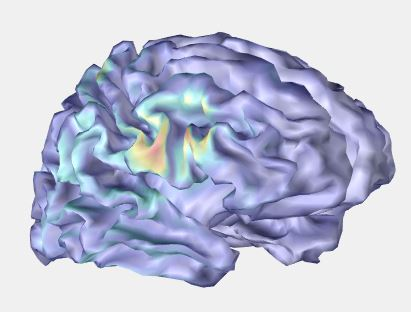
\includegraphics[width=1.0\textwidth]{casti/implementace/sourceReconstruction/render.jpg}
\caption{Příklad výsledku inverzní úlohy, výsledky vykresleny do skleněného mozku a do modelu mozku}
\label{prikladVysledku}
\end{figure}

Pokud není uživatel s výsledkem inverzní úlohy spokojen, může výpočet inverzní úlohy opakovat, použít jiné parametry, zvolit optimální frekvenční pásmo nebo vybrat jiný časový interval. V případě, že je uživatel s výsledky spokojený, může výsledky promítnout přímo do MRI snímků pacientovy hlavy pomocí tlačítka Image.
 
\begin{figure}[!h]
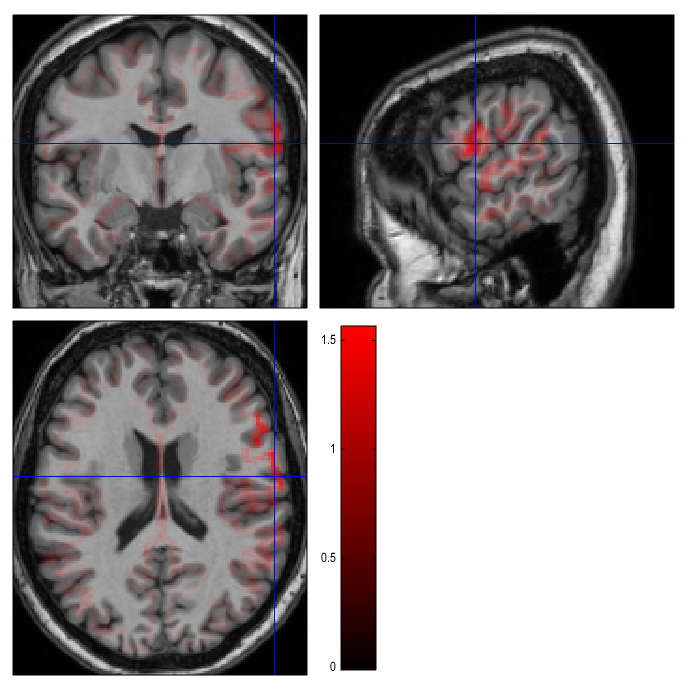
\includegraphics[scale = 0.4]{casti/implementace/sourceReconstruction/vysledek.png}
\caption{Příklad výsledku inverzní úlohy vykresleného do MRI snímku pacienta}
\label{vysledkyMRIsnimek}
\end{figure}

\subsubsection{Batch editor}
Aplikaci inverzní úlohy je možné provést využitím Batch editoru SPM12 toolboxu, provedením operací nazvaných Head model specification a Source inversion. První funkce definuje přímou úlohu, druhá vypočte inverzní úlohu podle zadaných specifikací.

Výhodou tohoto přístupu je možnost automatizace výpočtu, která se hodí v~případech, kdy je nutné zpracovat více případů podobného typu. Nevýhodou je ovšem nemožnost individuálně přistupovat ke každému případu a~kontrolovat správnosti mezikroků. 

Přístup, který jsem shledal nejlepším, je využití kombinace obou, grafického rozhraní i Batch editoru. Automatizuji proces předzpracování dat a~specifikace přímé úlohy pomocí Batch editoru, dále však zpracovávám případ individuálně pomocí grafického rozhraní. Zkontroluji, zda je model hlavy v pořádku, dále vypočítám inverzní úlohu a upravuji její parametry na základě získaných informací. Ve chvíli, kdy jsem s výsledkem spokojen, mohu z~grafického rozhraní pohodlně vykreslit výsledky do MRI snímků. 


\subsubsection{Obalující funkce }
Abych uživatelům SPM Motol toolboxu umožnil jednoduše aplikovat tento postup, naimplementoval jsem obalující funkci jménem \textbf{InversionStart}, jejímž vstupem jsou pouze cesty k EEG a MRI souborům a vstupní proměnné, definující délku okna, které bude použito při epochingu a indexy událostí určených ke zpracování. Díky této funkci je aplikace inverzní úlohy otázkou použití jediné funkce, která se postará o veškeré předzpracování, nadefinuje model pacientovy hlavy, provede koregistraci a vypočte prvotní inverzní úlohu. Uživatel je poté postaven pouze před úkol zlepšovat parametry inverzní úlohy, dokud není spokojený s výsledkem (může například porovnat výsledky metod, zda některá neukáže velmi odlišný výsledek, nebo může upravit uvažované frekvenční pásmo na základě znalosti signálu).

Naimplementoval jsem také podobnou funkci \textbf{InversionStartNoPreprocessing}. Od předcházející funkce se liší pouze tím, že neprovádí předzpracování vstupních dat. Tato funkce je vhodná pro případy, kdy předzpracování provede jiný software, například detektor grafoelementů (jehož výstupem mohou být již zprůměrované grafoelementy hrot-vlna).



%!TEX ROOT=../../Diplomka.tex

\chapter{Aplikace inverzních úloh}

\section{Porovnání metod inverze SPM12}
V SPM12 toolboxu je naimplementováno 5 algoritmů nedourčených modelů inverzní úlohy (GS, MSP, COH, IID a EBB). Abychom byli schopni metody porovnat, vytvořil jsem několik syntetických datových souborů, které obsahují data, o nichž vím, kde se nachází zdroj jejich aktivity. Syntetická data jsou generována pomocí přímé úlohy, na zvolené souřadnice jsou umístěny proudové dipóly, které generují zvolený průběh proudu. Následně je vypočteno, jak se tyto proudy propagují na skalp modelu a jaké potenciály jsou zaznamenány elektrodami. Funkce pro generování syntetických dat je součástí v SPM12 toolboxu. 

Proces vytváření syntetického datového souboru využívá již existujícího datového souboru s definovanou přímou úlohou, kde jednoduše nahradí označené události nově vypočtenými EEG průběhy se zvolenou úrovní Gaussovského šumu. Datových souborů, ze kterých jsem mohl vycházet, bylo k dispozici několik, vždy jeden od zpracovávaného případu. Náhodně jsem zvolil datový soubor pacienta P110 se 168 označenými událostmi jako výchozí. 

\subsection{Generování syntetických dat}
Vygeneroval jsem celkem 5 scénářů pro porovnání algoritmů inverzních úloh, na nichž jsem následně provedl výpočet inverzní úlohy dostupnými algoritmy:

\begin{itemize}
\item Zdroj v levé hemisféře na pozici [-52, -25, 9] generující průběhy o frekvenci 10 Hz, SNR nastaveno na 0 dB, viz obrázek \ref{scenar1}
\begin{figure}[!h]
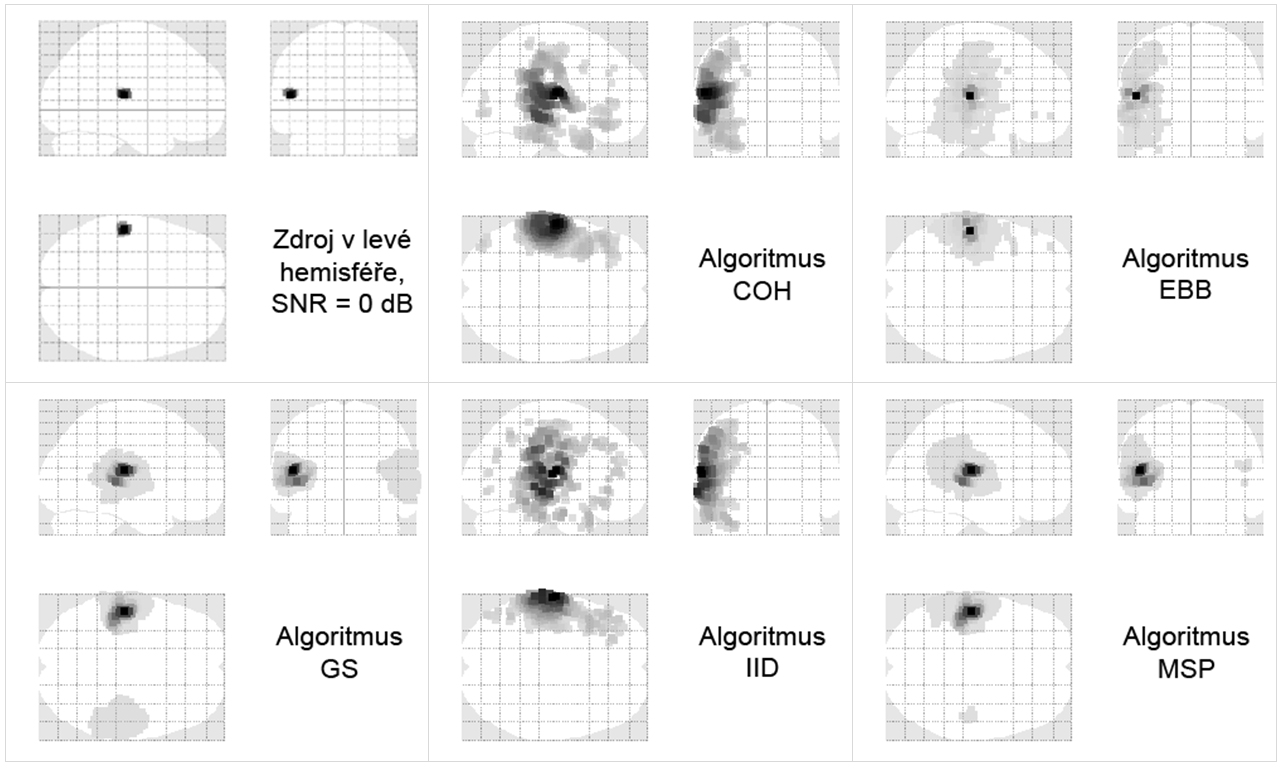
\includegraphics[width=1.0\textwidth]{casti/aplikace/porovnani/scenar1.png}
\caption{Výsledky lokalizace zdroje v levé hemisféře}
\label{scenar1}
\end{figure}

\item Zdroj v pravé hemisféře na pozici [52, -25, 9] generující průběhy o~frekvenci 20 Hz, SNR 0 dB, viz obrázek \ref{scenar2}
\begin{figure}[!h]
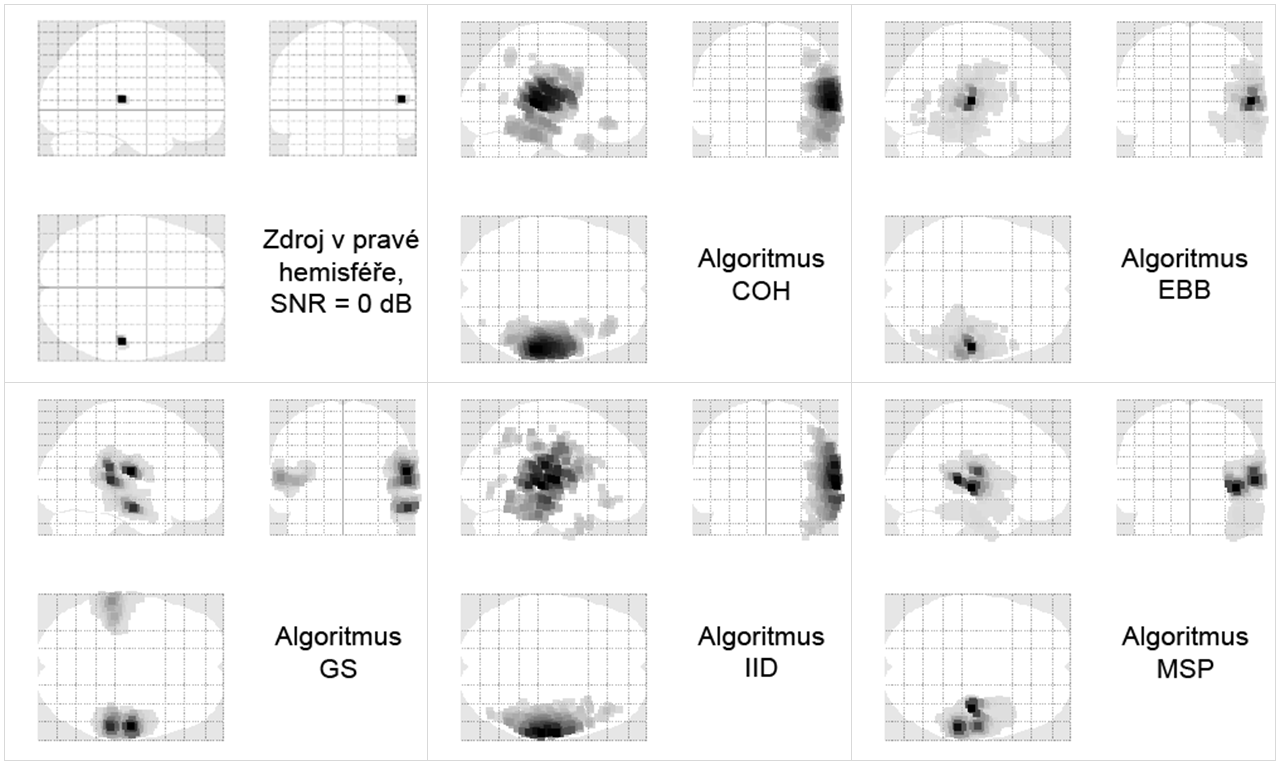
\includegraphics[width=1.0\textwidth]{casti/aplikace/porovnani/scenar2.png}
\caption{Výsledky lokalizace zdroje v pravé hemisféře}
\label{scenar2}
\end{figure}

\item Kombinace předchozích zdrojů v levé a pravé hemisféře, SNR = 10 dB, viz obrázek \ref{scenar3}
\begin{figure}[!h]
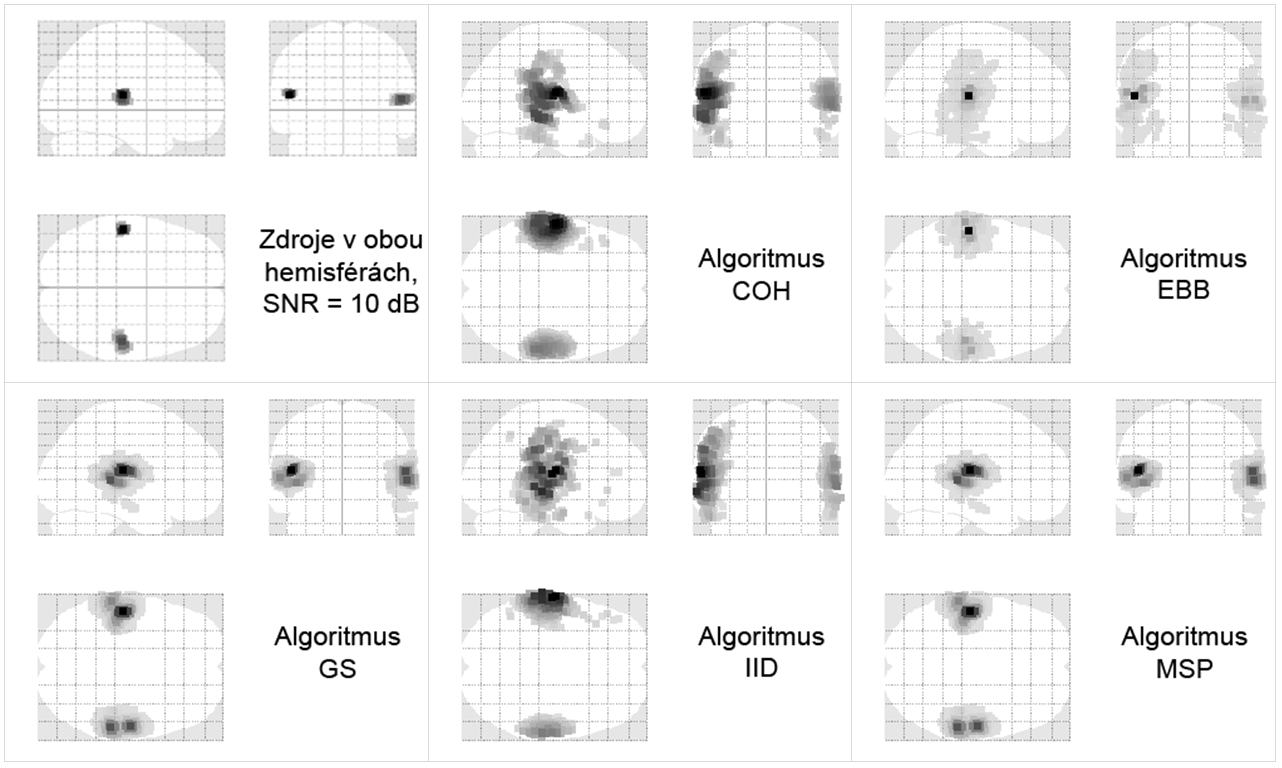
\includegraphics[width=1.0\textwidth]{casti/aplikace/porovnani/scenar3.png}
\caption{Výsledky lokalizace zdroje v pravé i levé hemisféře, při SNR 10 dB}
\label{scenar3}
\end{figure}

\item Kombinace zdrojů s hladinou SNR 0 dB, viz obrázek \ref{scenar4}
\begin{figure}[!h]
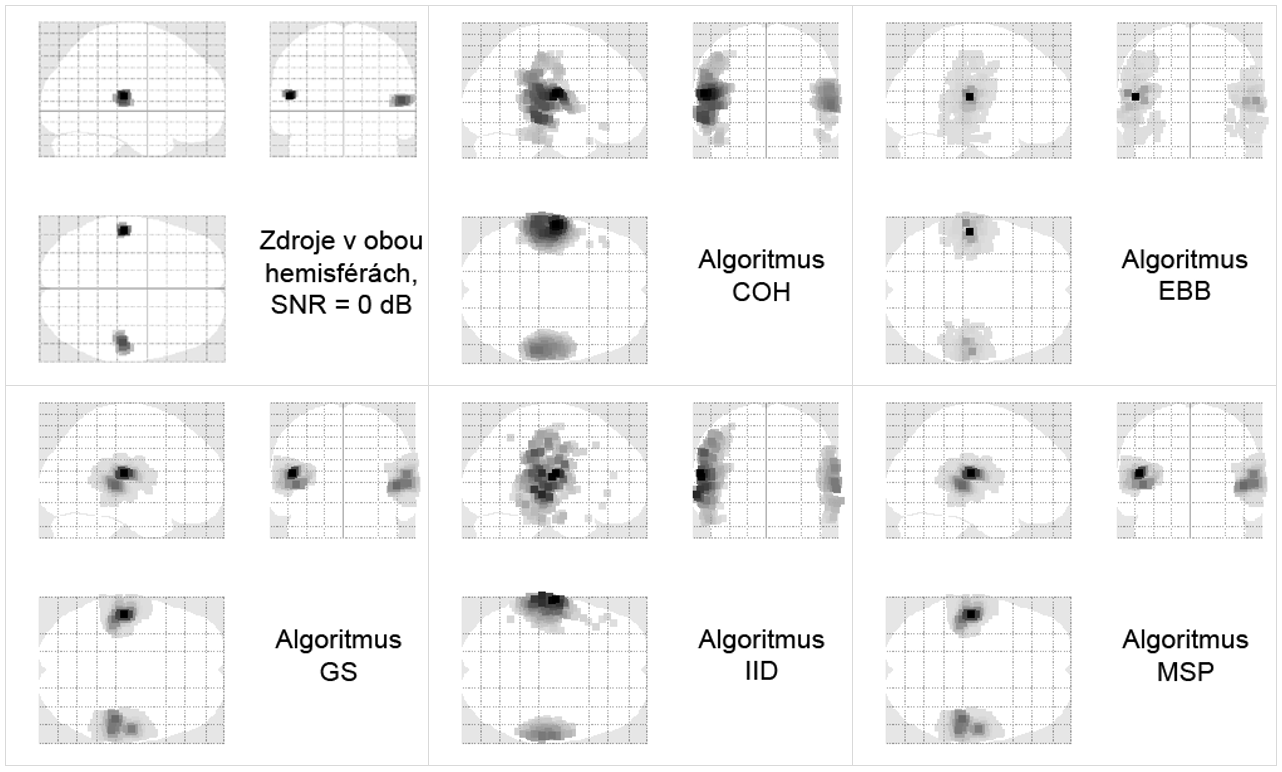
\includegraphics[width=1.0\textwidth]{casti/aplikace/porovnani/scenar4.png}
\caption{Výsledky lokalizace zdroje v pravé i levé hemisféře, při SNR 0 dB}
\label{scenar4}
\end{figure}

\item Kombinace zdrojů s hladinou SNR -10 dB, viz obrázek \ref{scenar5}
\begin{figure}[!h]
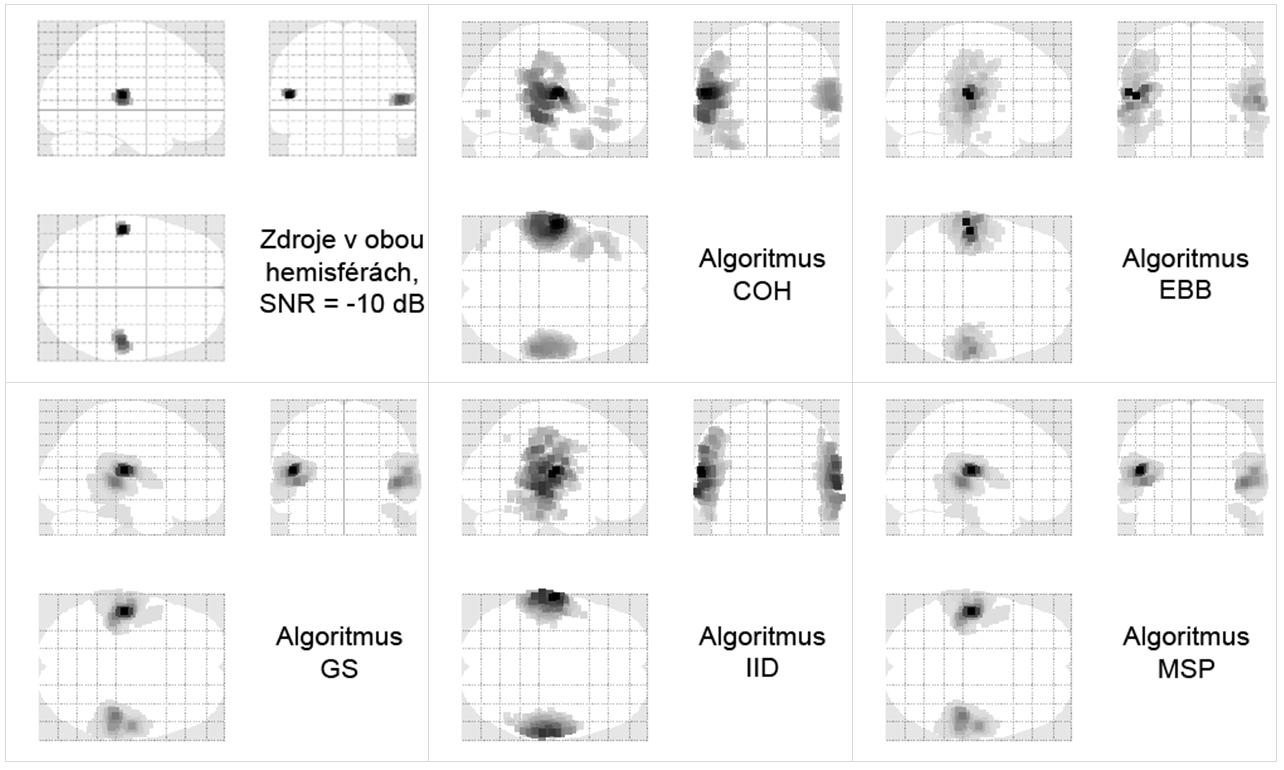
\includegraphics[width=1.0\textwidth]{casti/aplikace/porovnani/scenar5.png}
\caption{Výsledky lokalizace zdroje v pravé i levé hemisféře, při SNR -10 dB}
\label{scenar5}
\end{figure}

\end{itemize}


\subsection{Shrnutí výsledků}
Z těchto scénářů jsem vypočetl průměrné lokalizační chyby jednotlivých algoritmů. Jsou rozepsány v tabulce \ref{prumerneChyby}.

\begin{table}
\begin{ctucolortab}
\begin{tabular}{lp{1.2cm}p{1.2cm}p{1.2cm}p{1.2cm}p{1.2cm}}
\bfseries Algoritmus & COH	& EBB	& GS	& IID	& MSP \\
\Midrule
\bfseries Chyba lokalizace [mm] & 12,7	& 3,7	& 7,8	& 15,5	& 8,7
\end{tabular}
\end{ctucolortab}
\caption{Průměrné chyby lokalizace algoritmů inverzních úloh SPM12 toolboxu}
\label{prumerneChyby}
\end{table}

Z výsledků je možné vyvodit několik závěrů. Metody COH a IID mají tendenci promítat zdroj aktivity k povrchu mozku. U metody IID jsem tuto vlastnost očekával (viz teorie, \ref{minimumNorm}), u metody COH měla však být tato vlastnost kompenzována vhodným váhováním. Algoritmy GS a MSP dávají velmi podobné výsledky, i když MSP je oproti GS výpočetně mnohem náročnější (výpočet GS trvá desítky sekund, výpočet MSP zabere několik hodin). Všechny metody jsou robustní a dávají správné výsledky i v případě, že jsou jednotlivé události velmi zarušené. Důležitou roli zde hraje proces průměrování, ve výsledném signálu je šum dobře potlačen. Výsledky algoritmu EBB jsou velmi fokální, když jsou data generována ze dvou zdrojů, EBB bezpečně najde jeden z nich, druhý potlačí. Tento algoritmus je zároveň nejcitlivější na rušení.


\section{Aplikace inverzních úloh na reálná data}
Pro ověření použitelnosti SPM Motol toolboxu v praxi jsem naimplementované funkce použil při zpracovávání několika případů pacientů. Na případech jsem spolupracoval s pracovníky nemocnice Motol, kteří EEG data naměřili, a s konzultantem Ing. Petrem Ježdíkem, Ph.D.  Převážně se jedná o~zpracování somatosenzorických evokovaných potenciálů, které byly měřeny na epileptických pacientech během několikahodinového snímání. Zpracoval jsem ale i případ epilepsie pacienta.

\subsection{Měření reálných dat}
Měření high density EEG dat v nemocnici Motol provádí MUDr. Adam Kalina a proces měření probíhá následovně. Epileptický pacient se ráno dostaví do nemocnice, kde mu je nasazena čepice, která určuje rozložení elektrod. Za pomoci zdravotní sestry jsou elektrody nagelovány tak, aby byl zajištěn kontakt elektrody a skalpu hlavy, ale zároveň tak, aby nedošlo ke vzniku solných můstků. Následuje snímání pozic elektrod kamerovým systémem. Pacient je 2 hodiny monitorován v bdělém stavu, v tomto období probíhá kognitivní testování. Následují další 2 hodiny monitorace pacienta v leže, pokud možno ve spánku, kdy měření nebývá zatíženo svalovými artefakty. Poslední fází je měření somatozensorických evokovaných potenciálů. Pacient je přesunut do křesla, je mu podložena ruka dekou a MUDr. Kalina začne hledáním nervus medianus pomocí krátkých proudových stimulů. Hledání probíhá na spodní straně zápěstí polohováním dvou elektrod a pozorováním odezvy pacientovy ruky (očekávají se záškuby palce). Upravována je také amplituda stimulů tak, aby záškuby palce byly dostatečně silné a zároveň aby vyšetření nebylo pro pacienta bolestivé. Po nalezení potřebné polohy elektrod a amplitudy stimulů probíhá měření 512 somatosenzorických evokovaných potenciálů se stimulační frekvencí 2 Hz. Proces měření je proveden nejdříve na levé a poté na pravé ruce. Po dokončení této procedury je pacient propuštěn domů. \cite{67}

I když jsou pacienti instruováni, aby se snažili zůstat v klidu a uvolnili svalstvo, aby v záznamu nevznikaly zbytečné artefakty, často se tak neděje. Pacienti se po chvíli začínají nudit a převalují se na posteli. Pro vyhodnocování ložiska epilepsie jsou proto nejvhodnější data, naměřená při spánku, kdy je pacient uvolněný. Podobný problém provází i měření evokovaných potenciálů. Měření je zajímavé, pacient jej sleduje, přičemž se předkloní, aby dobře viděl, tím ale způsobí tonus krčních svalů a svalové artefakty v záznamu. Pokud se svalové artefakty z oblasti krku vyskytují po celou dobu měření somatosenzorických evokovaných potenciálů, průměrování se může stát méně účinným, protože se již nejedná o náhodnou aktivitu.

Pro měření EEG dat je využíván systém Asa-lab, skládající se ze dvou 128 kanálových zesilovačů a čepice s digitizérem od společnosti ANT Neuro. \cite{67}

\subsection{Lokalizace zdroje SEP}
Ideou stojící za prováděním somatosenzorických evokovaných potenciálů během zkoumání ložiska epilepsie je, že umožňují otestovat výsledky inverzní úlohy u konkrétního pacienta, protože u evokovaných potenciálů známe místo a čas, kde se má mozková aktiva objevit.

\subsubsection{Výsledky}
Výsledky byly vypočteny algoritmem LORETA (COH) ve frekvenčním pásmu 1 až 150~Hz, data byla převzorkována na frekvenci 1024 Hz. Využil jsem algoritmu LORETA, protože se v článcích, porovnávajících různé algoritmy umisťoval na prvních příčkách. Vlastní porovnání jsem prováděl až po evaluaci somatosenzorických evokovaných potenciálů.


\paragraph{Pacient P99}
U tohoto pacienta jsou k dispozici pouze data somatosenzorických evokovaných potenciálů levé ruky. Při stimulaci pravé ruky byl vyvolán záchvat (kvůli epileptickému ložisku blízko gyrus postcentralis levé hemisféry) a měření bylo přerušeno.

Ve výsledcích dostupných evokovaných potenciálů je hlavním zdrojem aktivity gyrus postcentralis, objevují se také dlouhodobě přetrvávající ložiska v okcipitální a frontální oblasti, která jsou pravděpodobně způsobena artefakty krčních a očních svalů. Další, méně výrazná, ložiska aktivity, která se objevují blízko primární senzitivní oblasti směrem k frontálnímu laloku, by mohla být způsobena primární a sekundární motorickou oblastí.
\begin{figure}[!h]
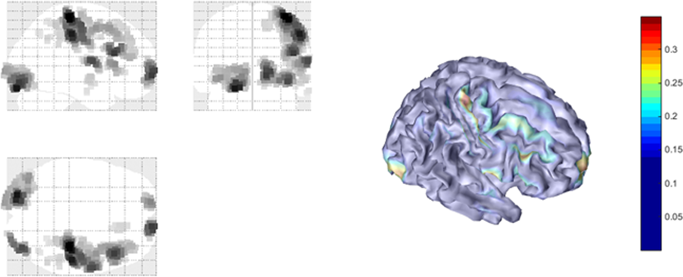
\includegraphics[width=1.0\textwidth]{casti/aplikace/sep/P99.png}
\caption{Výsledek inverzní úlohy evokovaných potenciálů pacienta P99}
\end{figure}

\paragraph{Pacient P109}
Hlavním zdrojem aktivity je primární senzitivní oblast pro ruku, kde aktivitu očekáváme. Ostatní zdroje aktivity jsou jen velmi slabými ložisky, kterým bych nepřikládal význam, protože jde pravděpodobně o náhodnou mozkovou aktivitu.

\begin{figure}[!h]
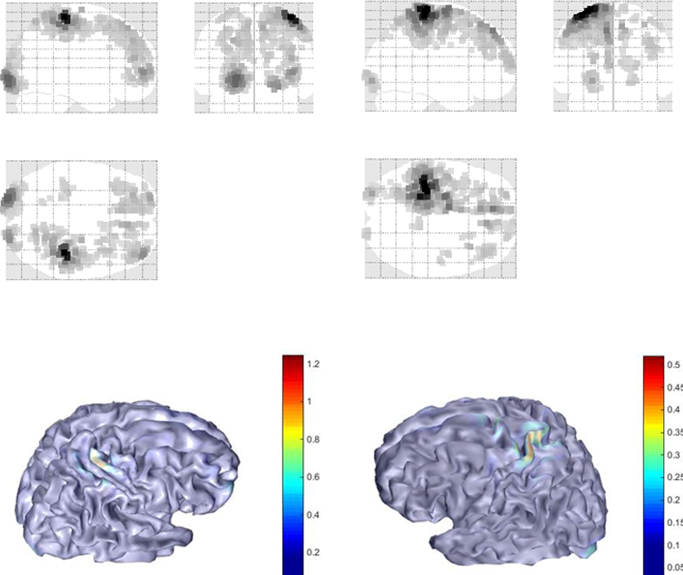
\includegraphics[width=1.0\textwidth]{casti/aplikace/sep/P109.png}
\caption{Výsledek inverzní úlohy evokovaných potenciálů pacienta P109}
\end{figure}

\paragraph{Pacient P110}
Ložiska aktivity jsou v tomto případě opět na očekávaném místě, ostatní zdroje jsou zanedbatelné.

\begin{figure}[!h]
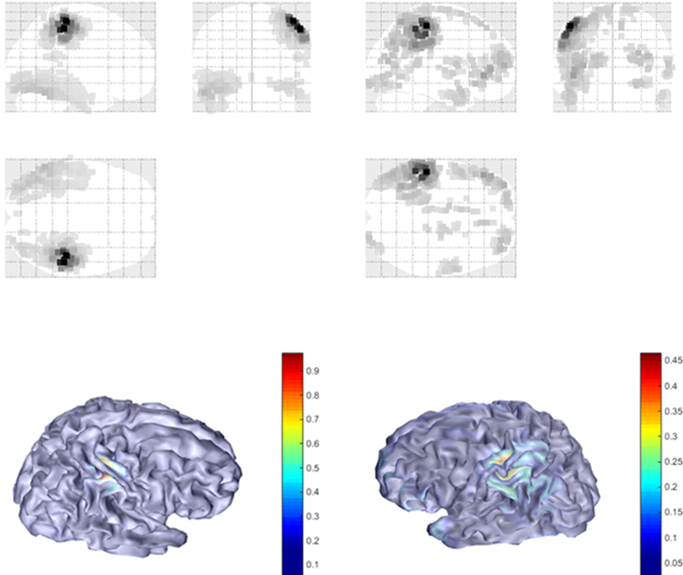
\includegraphics[width=1.0\textwidth]{casti/aplikace/sep/P110.png}
\caption{Výsledek inverzní úlohy evokovaných potenciálů pacienta P110}
\end{figure}

\paragraph{Pacient P113}
V tomto případě, u somatosenzorických evokovaných potenciálů pravé ruky, se opět objevuje silný dlouhodobý zdroj aktivity v okcipitální oblasti, opět asi způsoben svalovým tonem. Můžeme také pozorovat dvě ložiska v obou hemisférách ve frontální laloku. Pravděpodobně jde o jedno ložisko, které je chybně interpretováno inverzní úlohou. Toto ložisko se objevuje během stejného časového intervalu jako aktivita v gyrus postcentralis.
V~případě levé ruky se neobjevuje nic neočekávaného.
Výsledky jsou vykresleny v~obrázku \ref{sepP113}.


\paragraph{Pacient P114}
V případě evokovaných potenciálů levé ruky se aktivita v~primární senzitivní oblasti nečekaně neobjevuje. Objevuje se v primární a~sekundární motorické oblasti, zasahuje však až do spánkového laloku. Bohužel nejsem schopen odůvodnit, proč k tomuto jevu došlo.
V případě měření prováděných za stimulace pravé ruky se již ložisko v gyrus postcentralis pro ruku objevuje, je ale zastíněno vyšší aktivitou gyrus postcentralis pro oblast obličeje.
Výsledky jsou vykresleny v obrázku \ref{sepP114}.

\paragraph{Shrnutí výsledků}
Ve výsledcích somatosenzorických evokovaných potenciálů u všech pacientů (vyjma pacienta P114 evokované potenciály levé ruky) je vidět aktivita na očekávaném místě v gyrus postcentralis.

V některých případech je vidět také aktivita v okcipitální oblasti a frontálním laloku, která přetrvává během celého časového okna. Je pravděpodobně způsobena artefakty krčních a očních svalů.

Občasně je také vidět ložisko aktivity, které nelze vysvětlit svalovými artefakty ani evokovanými potenciály. Taková ložiska ale přetrvávají jen několik časových vzorků, proto si myslím, že jde o náhodnou mozkovou aktivitu, kterou se nepodařilo odstranit průměrováním.

V případě evokovaných potenciálů levé ruky pacienta P114 vidíme výsledek mimo očekávanou oblast, aktivita se objevila o několik centimetrů posunutá směrem k čelnímu laloku. 



\begin{figure}[!p]
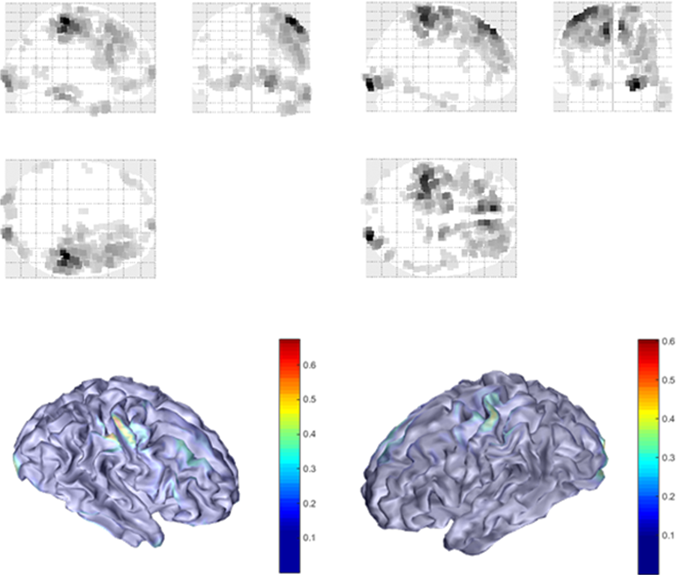
\includegraphics[width=0.9\textwidth]{casti/aplikace/sep/P113.png}
\caption{Výsledek inverzní úlohy evokovaných potenciálů pacienta P113}
\label{sepP113}
\end{figure}

\begin{figure}[!p]
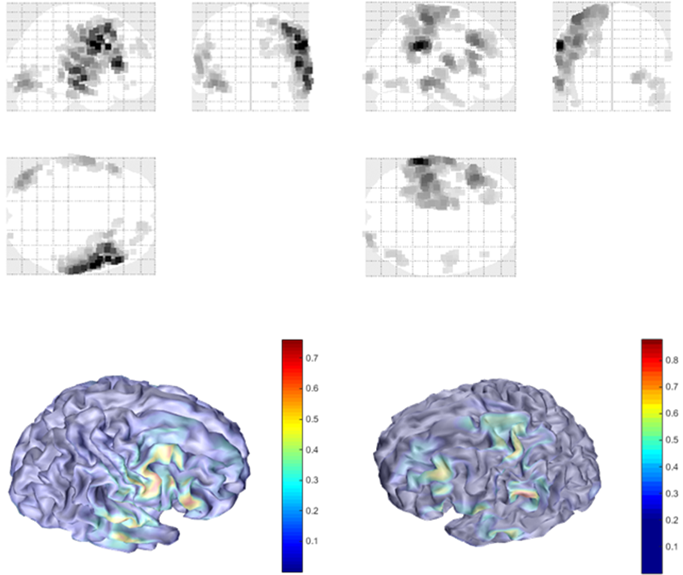
\includegraphics[width=0.9\textwidth]{casti/aplikace/sep/P114.png}
\caption{Výsledek inverzní úlohy evokovaných potenciálů pacienta P114}
\label{sepP114}
\end{figure}




\newpage
\subsection{Lokalizace zdroje epileptické aktivity pacienta P81}

\subsubsection{Tvorba dat}
Data pro analýzu epileptických grafoelementů hrot-vlna a výpočet inverzní úlohy připravil Ing. Petr Ježdík, Ph.D. Ze 110 minut high density záznamu o 256 elektrodách vybral celkem 45 minut záznamu ve spánku, které byly vhodné pro aplikaci automatické detekce komplexů hrot-vlna. Ostatní data obsahovala četné artefakty.

Na vybraná data epileptického pacienta byl aplikován jednokanálový detektor komplexů hrot-vlna, navržený Ing. Radkem Jančou, Ph.D. v článku \cite{70}. Nalezené grafoelementy jsou následně roztříděny do skupin (clusterů) pomocí PCA (Principal Component Analysis) algoritmu. Získané skupiny podobných průběhů jsou následně podrobeny průměrování, získáme tak 1,5 sekundy dlouhý vzorek EEG záznamu příslušného clusteru o 256 kanálech. Jednotlivé průběhy jsou podrobeny vizuální inspekci a jsou vybrány clustery, které skutečně obsahují komplexy hrot-vlna spojené s epilepsií (jiné skupiny mohou obsahovat falešné detekce, jde například o průměty EKG do kanálů EEG, o kterých víme, že jsou také detekovány detektorem; takový cluster je z analýzy vyřazen). Podrobnosti o procesu vytváření clusterů grafoelementů pomocí PCA budou zveřejněny v následujícím článku Ing. Radka Janči, Ph.D. \cite{75}

Nejvíce informací o ložisku epilepsie obsahuje hrot, vlna je pouze následnou odezvou. Hrot se v tomto případě nachází v čase 490 milisekund.
\begin{figure}[!h]
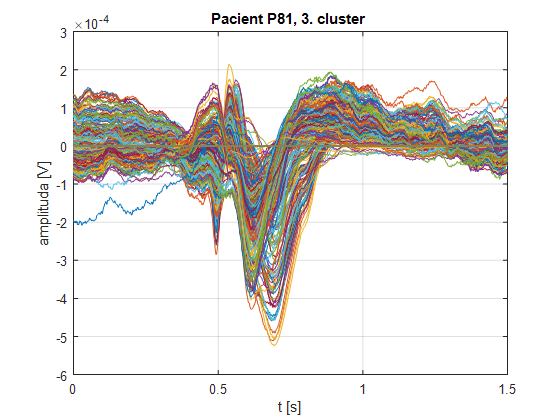
\includegraphics[width=1.0\textwidth]{casti/aplikace/epilepsie/prubehy.png}
\caption{Průměr z komplexů hrot-vlna pacienta P81}
\end{figure}

Ing. Petr Ježdík, Ph.D. také připravil analýzu nad prostorem elektrod, která je znázorněna na obrázku \ref{analyzaElektrod}. Skládá se z grafického vynesení četnosti detekovaných komplexů hrot-vlna za minutu (vyneseno v prvním sloupci), z~pozorovaných amplitud jednotlivých výbojů (druhý sloupec) a ze zobrazení času šíření vzruchu po detekovaném hrotu (sloupec vpravo). Jako vhodné pro aplikaci inverzní úlohy byly vybrány první dva clustery (první cluster v~prvním řádku obrázku \ref{analyzaElektrod}, druhý v druhém), které byly výstupem PCA.
\begin{figure}[!h]
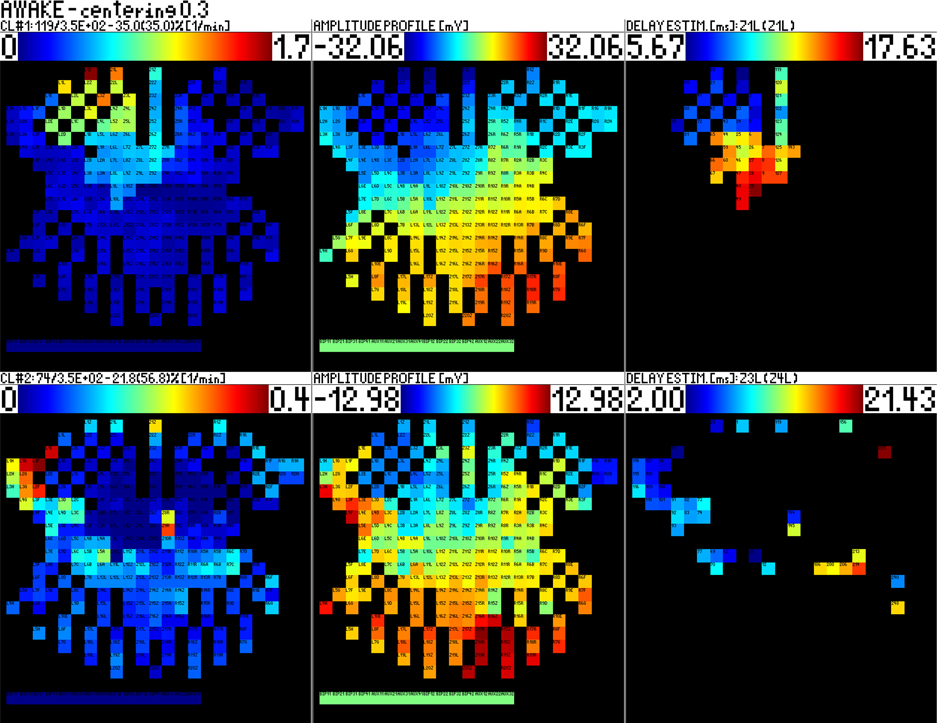
\includegraphics[width=1.0\textwidth]{casti/aplikace/epilepsie/analyza.png}
\caption{Analýza prostoru elektrod}
\label{analyzaElektrod}
\end{figure}

Z této analýzy jsme usoudili, že se očekávané ložisko epileptických výbojů nachází ve frontálním laloku levé hemisféry. V tomto místě bylo detekováno nejvíce komplexů hrot-vlna a odtud se výboj šířil dál do mozku. Výsledek lokalizace prvního clusteru jsem očekával v čelní části levé hemisféry. Ložisko, podle druhého clusteru, by se mělo nacházet v levé hemisféře, několik centimetrů pod Brocovým centrem řeči.
 
Parametry inverze jsem nastavil tak, aby bylo bráno v potaz frekvenční pásmo 16 až 128 Hz. To mi umožní zachovat vysoké frekvence komplexu hrot-vlna a zároveň potlačit pomalé průběhy s vysokou energií, které se mohou jevit jako hlavní ložiska aktivity, i když nemají s epilepsií nic společného. Pro inverzi jsem využil algoritmu LORETA (v SPM12 toolboxu pod zkratkou COH).

\newpage
\subsubsection{Výsledky}

\paragraph{1. cluster}
Na výsledných obrázcích je vidět vykreslení do skleněného mozku (vlevo nahoře), kde jsem označil strany mozku, aby nedošlo k nedorozumění. V pravé horní části je vidět průběh odhadnutý virtuální elektrodou v místě nejvyšší aktivity. Spodní obrázky vykreslují výsledky do trojrozměrného modelu pacientova mozku a do MRI snímků.

\begin{figure}[!h]
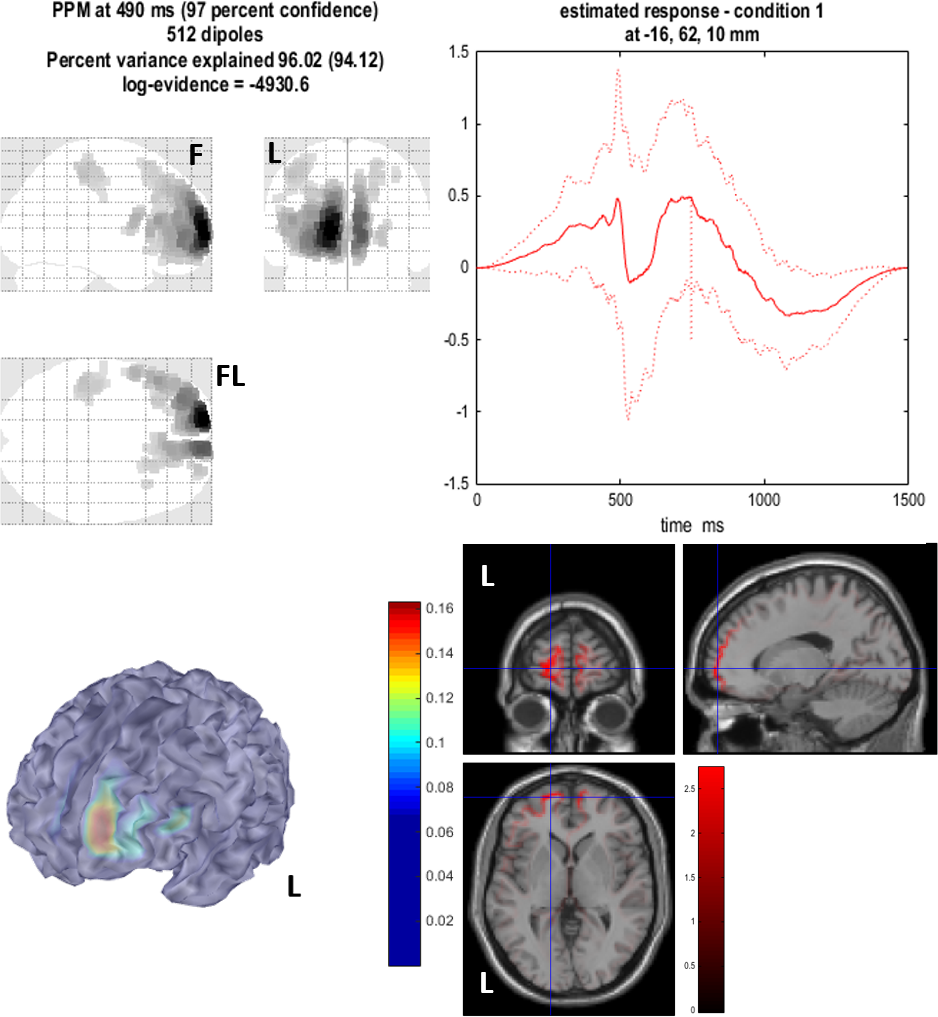
\includegraphics[width=1.0\textwidth]{casti/aplikace/epilepsie/1cl.png}
\caption{Výsledek inverzní úlohy epileptického pacienta P81, 1. cluster}
\end{figure}


\paragraph{2. cluster}
Aktivita tohoto clusteru se objevuje na předpokládaném místě pod Brocovým centrem řeči. Výsledky jsou zobrazeny v obrázku \ref{epilepsieCluster2}.

\begin{figure}[!h]
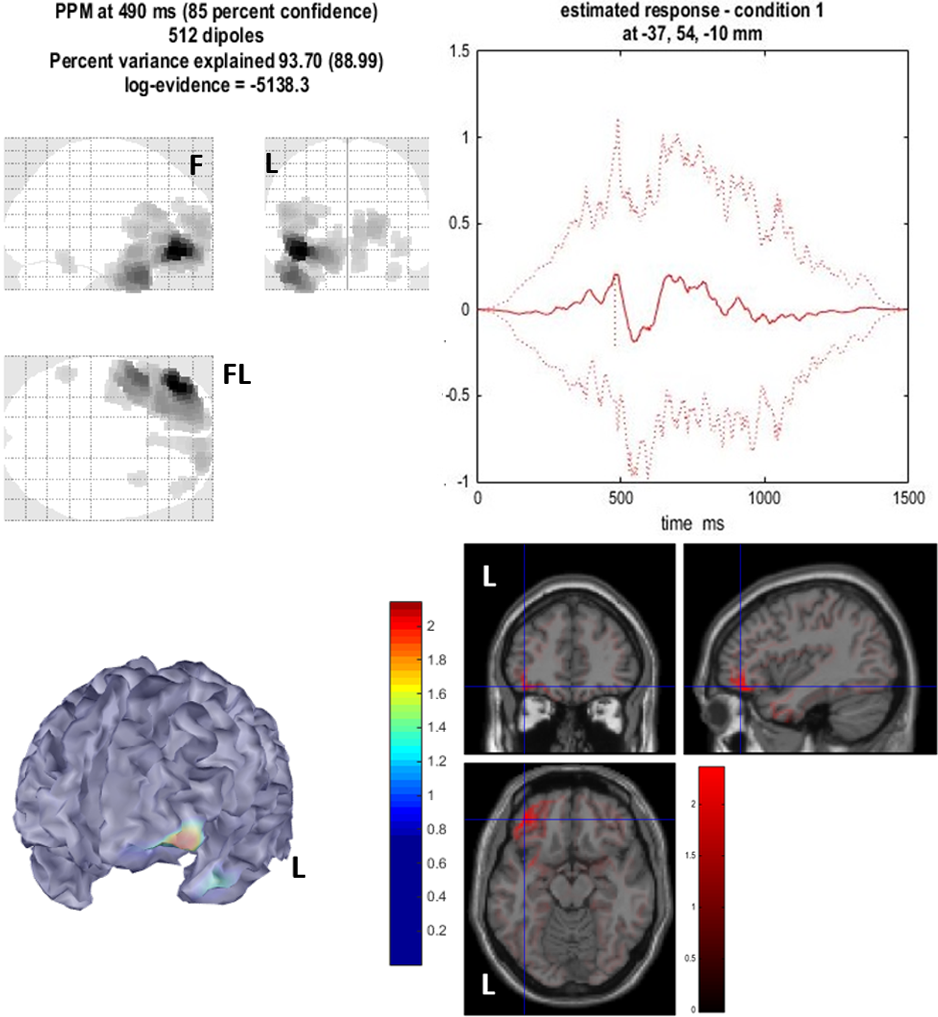
\includegraphics[width=1.0\textwidth]{casti/aplikace/epilepsie/2cl.png}
\caption{Výsledek inverzní úlohy epileptického pacienta P81, 2. cluster}
\label{epilepsieCluster2}
\end{figure}

\paragraph{3. cluster}
Tento cluster, také vhodný pro aplikaci inverzní úlohy, byl nalezen při dalším zpracování algoritmem PCA. Očekávám podobný výsledek jako u~prvního clusteru. Výsledky jsou zobrazeny v obrázku \ref{epilepsieCluster3}.

\begin{figure}[!h]
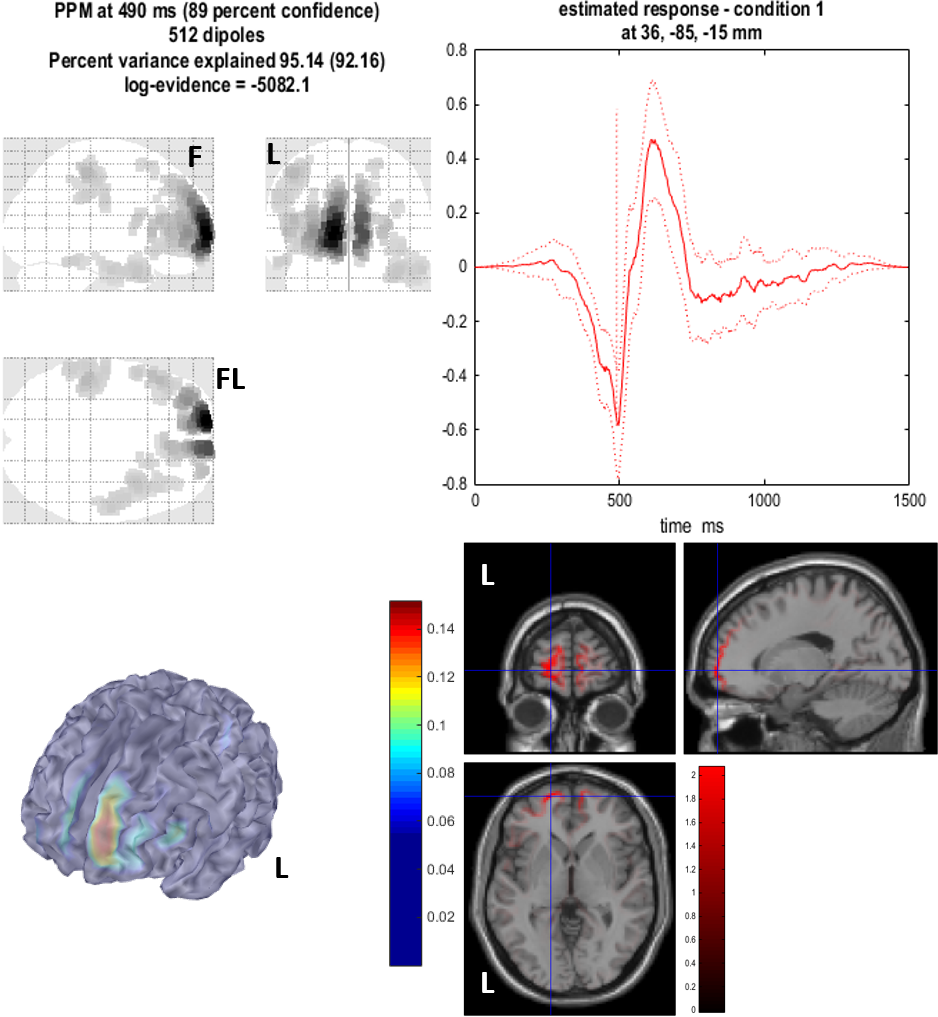
\includegraphics[width=1.0\textwidth]{casti/aplikace/epilepsie/3cl.png}
\caption{Výsledek inverzní úlohy epileptického pacienta P81, 3. cluster}
\label{epilepsieCluster3}
\end{figure}

\paragraph{Shrnutí}
Výsledek inverze potvrzuje očekávání předchozí analýzy. Hlavní ložisko aktivity se nachází ve frontálním laloku levé hemisféry. Ložisko je nejlépe zřetelné v čase 490 ms, tedy v čase, kde se nachází hrot komplexu hrot-vlna. Výsledné ložisko vypadá, jako by zasahovalo také do druhé hemisféry, ve skutečnosti tomu tak není, inverzní metody neumí rozlišovat mezi funkčně odlišnými celky, jako jsou například hemisféry. Takové chyby je možné vyloučit vhodnou interpretací výsledků. 

%!TEX ROOT=../../Diplomka.tex

\chapter{Závěr}
Epilepsie je mozkové onemocnění projevující se výpadky normální mozkové aktivity. Způsob léčby antiepileptiky je zaměřen spíše na léčbu projevů, než na odstranění příčiny onemocnění. Závažný problém nastává v případě farmakorezistentních pacientů, kdy léky účinkují nedostatečně nebo vůbec. Pro některé pacienty je možnou léčbou chirurgické odstranění epileptogenní zóny, tuto zónu je však nutné správně lokalizovat. Teorie určování zdroje aktivity v mozku z elektroencefalografických nebo magnetoencefalografických dat prodělala v posledních dekádách rozmach. Byly vyvinuty mnohé algoritmy, které se snaží zdroje lokalizovat pomocí různých předpokladů, založených na anatomických, fyziologických a biofyzikálních znalostech. Tyto algoritmy jsou souhrnně nazývány inverzními úlohami a umožňují lokalizovat zdroje aktivity neinvazivně, ze skalpového EEG. Z rozšíření inverzních úloh do klinické praxe by mohlo profitovat mnoho epileptických pacientů. Tato motivace mě vedla k~tomu, abych se v rámci své diplomové práce seznámil s teorií epilepsie, přímých a inverzních úloh, a získané znalosti následně aplikoval při vytváření nástrojů, které by pracovníkům nemocnice Motol umožnily jednoduše aplikovat inverzní úlohu.

Vytvořil jsem nadstavbu Matlab toolboxu SPM12, kterou jsem pojmenoval SPM Motol toolbox. Software umožňuje jednoduché využití inverzních úloh. Výpočet začíná automatizovaným předzpracováním, které se skládá z~opravy reference zesilovačů, filtrace nevhodných frekvenčních pásem, odstranění izolinie, selekce časových oken okolo událostí v~datech a~jejich následného průměrování a vytvoření datového souboru kompatibilního s SPM12. Následuje vytvoření modelu pacientovy hlavy, koregistrace elektrod s MRI a~aplikace inverzní úlohy podle výběru uživatele. Celý tento proces je možné spustit jedinou funkcí \texttt{InversionStart}, která v sobě volá další funkce obsluhující jednotlivé kroky. Výsledky inverze je možné generovat do skleněného mozku, do modelu mozku nebo přímo do MRI snímků. 

Aby bylo možné udělat si představu o praktické přesnosti výsledků dostupných algoritmů inverzních úloh, vygeneroval jsem syntetická data se známou polohou zdroje aktivity, která k tomuto účelu posloužila. Z poloh výsledků algoritmů jsem vypočetl průměrné chyby lokalizace. Nejvyšší přesnosti dosáhl algoritmus EBB, který ovšem občas potlačuje některá ložiska. Naopak nejhorších výsledků dosáhl algoritmus IID kvůli své jednoduchosti a vlastnosti promítat zdroje aktivity k povrchu mozku.

Zpracoval jsem měření somatosenzorických evokovaných potenciálů u pěti testovaných pacientů pro ověření aplikovatelnosti inverzních úloh na reálná data a použitelnost v praxi. Výsledky pacientů P99, P109, P110 a P113 vyšly přesně v očekávaném místě, v gyrus postcentralis kontralaterálně ke stimulované končetině, u pacienta P114 se odezva na evokované potenciály objevila o několik centimetrů posunutá směrem k čelnímu laloku.

V závěru jsem zpracoval kazuistiku epileptického pacienta P81. Bylo lokalizováno potenciální epileptogenní ložisko interiktálních výbojů ve frontálním laloku levé hemisféry. Výsledky inverzní úlohy korelují s předpoklady o~poloze ložiska, která byly získány během dalších analýz.

Mezi omezení SPM Motol toolboxu patří způsob, kterým vytváří modely mozku. Modely jsou vytvářeny geometrickou transformací standardního MNI mozku, ten je však průměrem snímků pacientů s celým mozkem. Toolbox je tedy nevhodný pro zpracovávání případů pacientů s již resekovanými mozky, u kterých ale záchvaty přetrvaly. Model hlavy takového pacienta bude deformovaný a nebude tak splňovat předpoklady pro úspěšnou aplikaci inverzního problému.

Popsané omezení by mohlo být odstraněno během následujícího vývoje SPM Motol toolboxu implementací nového způsobu vytváření modelů hlav pacientů. SPM Motol toolbox je také možné rozšířit o další existující algoritmy inverzních úloh, software také dává prostor pro vývoj zcela nových algoritmů inverzních úloh.

V současnosti SPM Motol toolbox úspěšně využívá Ing. Petr Ježdík, Ph.D. při zpracovávání kazuistik epileptických pacientů nemocnice Motol, toolbox však může využít každý, kdo má přístup k prostředí Matlab. Doufám, že se software bude postupně rozšiřovat do dalších nemocnic a pomáhat epileptickým pacientům nejenom v Motole.



\appendix
\printindex
\appendix
\bibliographystyle{plain}
\bibliography{casti/citace/citace}

\chapter{Seznam použitých zkratek}
\begin{table}[!htb]
\centering
\caption{Seznam použitých zkratek}
\label{my-label}
\begin{tabular}{ll}
AP & Akční potenciál \\
CT & Počítačová tomografie \\
EBB & Empirical Bayes beamformer \\
EEG & Elektroencefalografie \\
EKG & Elektrokardiografie \\
EMG & Elektromyografie \\
EOG & Elektrookulografie \\
ERP & Event related potencial \\
FEM & Metoda konečných prvků \\
fMRI & Funkční MRI \\
GS & Greedy search \\
LORETA &  Laplacian weighted minimum norm algorithm \\
M/EEG & Magnetoencefalografie a elektroencefalografie \\
MEG & Magnetoencefalografie \\
MN & Minimum norm \\
MRI & Magnetická rezonance \\
MSP & Multiple sparse priors \\
NIfTI & Neuroimaging Informatics Technology Initiative file format \\
PET & Pozitronová emisní tomografie \\
PSP & Postsynaptický potenciál \\
SEP & Somatosenzorické evokované potenciály \\
SPECT & Jednofotonová emisní tomografie \\
SPM & Statistical Parametric Mapping \\
WMN & Weighted minimum norm
\end{tabular}
\end{table}

\chapter{Struktura přiloženého CD}
\begin{forest}
  for tree={
    grow'=0,
    child anchor=west,
    parent anchor=south,
    anchor=west,
    calign=first,
    edge path={
      \noexpand\path [draw, \forestoption{edge}]
      (!u.south west) +(7.5pt,0) |- node[fill,inner sep=1.25pt] {} (.child anchor)\forestoption{edge label};
    },
    before typesetting nodes={
      if n=1
        {insert before={[,phantom]}}
        {}
    },
    fit=band,
    before computing xy={l=15pt},
  }
[
  [SPM motol toolbox
    [Examples
		[Batches
			[...]
		]
		[STARTepilepsy.m]
		[STARTsep.m]
		[Test\_zaznamu\_spektrum.m]
		[Testovani\_zaznamu.m]
		[Vykresleni\_pozic\_elektrod.m]
    ]
    [MRIcron
		[mricron
			[...]
		]
		[Readme.txt]
	]
    [SPM Motol
			[spm12motol
				[MotolFunctions
					[...]
				]
				[...]
			]
			[Readme.txt]
			[SPM12Motol\_Installer.m]	
		]
  ]
  [Hrstka - DP - 2016.pdf]
]
\end{forest}

\ctutemplate{specification.as.chapter}

\end{document}
